%!TEX encoding = UTF-8 Unicode
%!TEX program = xelatex

\documentclass[doctor]{hnuthesis}
% \usepackage{subfigure}
\usepackage{amsmath}
\usepackage{algorithmicx,algpseudocode}
\usepackage{float}

\usepackage{amsthm} % for proof
\usepackage{setspace} % setstretch
\usepackage{graphicx} % resizebox
\usepackage{makecell} % for makecell 
\usepackage{multirow} % for table
\usepackage{multicol} % for table
\usepackage{pifont}
\usepackage{mathtools} % for \begin{multlined} also begin{align}
	
\usepackage{caption} % for subfigure error
\usepackage{subcaption} % for subfigure error
\usepackage{mathtools} % for ceil  & multilined
\usepackage{amsfonts} % for mathbb
\usepackage{balance} % for \balancea
\usepackage{ctex}
\usepackage[export]{adjustbox} 
% 学校代码
\hnucode{10532}
% 学校名称
\hnuname{湖南大学}
\enhnuname{Hunan University}
% 中图分类号
\clc{TP391}         
% 密级       
\secrettext{不保密}           

% 标题
\title{CSM-TopK:密度约束下的TopK连续子图匹配}
\entitle{CSM-TopK: Continuous Subgraph Matching with
TopK Density Constraints}
% 作者
\author{高楚楚}
\enauthor{Chuchu Gao}
% 学号
\authorid{S221000763}      
% 学院
\college{信息科学与工程学院}
% 专业
\major{计算机科学与技术} 
\enmajor{Computer Science and Technology}
%学士学位获得学校,年份
\enbachelor{B.E.~(Hefei University of Technology)2022}
% \enmaster{M.S.~(Hunan University)2020}
\endoctor{Master of engineering}
% 研究方向
\workon{子图匹配}
% 导师
\supervisor{周旭\ 教授}
\ensupervisor{Professor Xu Zhou}
% 论文提交、答辩日期
\submitdate{2025年05月08日}
\defensedate{2025年05月21日}
\endate{May, 2025}
% 答辩委员会主席
\chair{廖鑫}

\begin{document}
% 封面、原创性声明
\maketitle

% 摘要
%中文摘要
\begin{abstract}
	连续子图匹配(Continuous Subgraph Matching,CSM)是动态图分析中的一个重要问题。该问题要求在一个动态变化的图中,寻找与查询图同构的所有子图,并根据匹配结果进行后续分析。
	由于动态图中的边和节点会实时发生变化,传统的静态子图匹配方法难以应对这些变化。

	目前,现有的CSM方法在处理大规模动态图时存在一个突出的问题:当查询图较为简单时,通常会产生大量的匹配结果。
	对于数据分析人员而言,过多的匹配子图不仅增加了计算负担,而且可能导致有价值的信息被淹没。
	此外,许多现实世界中的图是加权图,如支付网络,其中每条边的权重代表交易金额。
	在分析过程中,边的权重通常对匹配结果的优先级产生重要影响。然而,现有的CSM方法大多忽略了这一因素,未能有效地将边权引入优化策略。

	针对上述问题,本文提出了一个新的研究问题——CSM-TopK,即在动态加权图中计算查询图的前k个密度最高的匹配结果,并证明该问题为NP难问题。本文的主要贡献如下:
	\begin{enumerate}[label=(\arabic*)]  
	\item 为了有效解决CSM-TopK问题,我们首先定义了一种星形结构子图,并通过查询图匹配序列中节点的一阶邻居关系来导出该星形子图。
	\item 在星形结构子图的基础上,我们设计了两种轻量级索引,分别为全局MWstar索引和局部MWstar索引。具体而言,全局MWstar维护每个特定星形结构子图的最大权重,并在子图搜索的过程中保持不变,利用该最大权重,我们可以提前计算匹配子图的最大密度上限,从而进行剪枝,减少搜索空间,提高子图匹配的效率。
	而局部MWstar则根据每个特定数据顶点的最大权重分布动态维护索引,其最大权重的密度上限更加紧凑,因此能够更快地减少不必要的计算。
	\item 为了进一步提高性能,本文还引入了一种查询相关的图压缩技术,该技术利用标签过滤方式过滤不可能的候选点,从而生成针对此查询图的压缩图。由于压缩图的规模远小于数据图,在此基础上进行星形结构索引的初始化以及更新,显著降低了匹配子图的密度上限,从而提高了整体的时间和空间效率。
  	\end{enumerate}

	通过在五个真实世界数据集上的广泛实验,结果表明,结合图压缩技术和MWstar索引的最终方法表现最佳,在插入/删除的时间效率上,该方法相比现有对比方法至少提高了两个数量级;在索引的空间效率以及时间效率上也远超其他方法。实验结果验证了本文提出解决方案的有效性。
	\keywords{连续子图匹配;动态图;剪枝策略;TopK密度}
\end{abstract}

%英文摘要
\begin{enabstract}
	Continuous Subgraph Matching (CSM) is an important problem in dynamic graph analysis. 
	The problem requires finding all subgraphs in a dynamically changing graph that are isomorphic to a given query graph, and performing further analysis based on the matching results. 
	Since edges and vertices in a dynamic graph change in real-time, traditional static subgraph matching methods struggle to cope with these changes.

    Currently, existing CSM methods face a prominent issue when handling large-scale dynamic graphs: when the query graph is simple, it often generates a large number of matching results. 
	For data analysts, an excessive number of matching subgraphs not only increases the computational burden but may also drown out valuable information. 
	Moreover, many real-world graphs are weighted, such as payment networks, where each edge’s weight represents the transaction amount. 
	During analysis, edge weights often significantly influence the priority of matching results. However, most existing CSM methods overlook this factor and fail to effectively incorporate edge weights into the optimization strategies.

	
	To address these challenges, the paper introduces a new problem called CSM-TopK, which aims to compute the top k matching results with the highest density for a given query graph on dynamic weighted graphs and proves that this problem is NP-hard. 
	The main contributions are as follows:
	\begin{enumerate}[label=(\arabic*)]  
		\item To efficiently solve the CSM-TopK problem, we first define a star-structured subgraph, which derives the star-structured subgraph using the first-order neighborhood relationships of the vertices in the query graph’s matching order.
		\item Based on the star-structured subgraph of the query graph, we design two lightweight indexes, namely the Global MWstar Index and the Local MWstar Index. 
		Specifically, the Global MWstar maintains the maximum weight of each specific star-structured subgraph, which remains unchanged during subgraph search. 
		Using this maximum weight, we can compute the upper bound of the maximum density for the matching subgraph in advance, enabling pruning to reduce the search space and improve matching efficiency. 
		In contrast, the Local MWstar dynamically maintains the index based on the maximum weight distribution of each specific data vertex. 
		Its maximum weight density upper bound is more compact, allowing for faster reduction of unnecessary computations.
		\item To further enhance performance, we also introduce a query-dependent graph compacted technique. 
		This technique uses label filtering to remove impossible candidate vertices, yielding the candidate subgraph specifically for the query graph. 
		The size of the candidate subgraphs is significantly smaller than the original data graph. 
		The initialization and updating of the star-structured index on the candidate subgraph substantially reduce the upper bound of the matching subgraph’s density, thereby improving both time and space efficiency.
		\end{enumerate}

		Extensive experiments on five real-world datasets demonstrate that the proposed method combining graph compression techniques and MWstar indexing performs the best. 
		In terms of time efficiency for insertions/deletions, it outperforms existing comparison methods by at least two orders of magnitude. 
		It also significantly exceeds other methods in both index space efficiency and time efficiency. 
		These experimental results validate the effectiveness of the proposed solution.
	\enkeywords{Continuous Subgraph Matching; Dynamic Graph; Pruning Strategy; TopK Density}
\end{enabstract}
% 目录
\tableofcontents
% 插图附表索引
\begingroup
    \renewcommand*{\addvspace}[1]{}
        \phantomsection
        \listoffigures
        \newpage

        \phantomsection
        \listoftables
        \newpage
\endgroup
%% The following content must be adapted for the final version
% paper-specific

%\newcommand\vldbdoi{XX.XX/XXX.XX}
%\newcommand\vldbpages{XXX-XXX}
%% issue-specific
%\newcommand\vldbvolume{15}
%\newcommand\vldbissue{1}
%\newcommand\vldbyear{2023}
%% should be fine as it is
%\newcommand\vldbauthors{\authors}
%\newcommand\vldbtitle{\shorttitle} 
%% leave empty if no availability url should be set
%\newcommand\vldbavailabilityurl{https://github.com/zmli6/csm-plus-plus}
%% whether page numbers should be shown or not, use 'plain' for review versions, 'empty' for camera ready
%\newcommand\vldbpagestyle{plain} 
% \newtheorem{definition}{\bf Definition}
\newcommand{\csmfolder}{./exp/}
\newcommand{\csmnewFig}{./exp/newFig/}
\newcommand{\tablefolder}{./tab/}
\newcommand{\picfolder}{./pics/}
\newcommand{\figs}{./figures/}


%\newcommand{\vldbblock}{
%%%% do not modify the following VLDB block %%
%%%% VLDB block start %%%
%\pagestyle{\vldbpagestyle}
%\begingroup\small\noindent\raggedright\textbf{PVLDB Reference Format:}\\
%\vldbauthors. \vldbtitle. PVLDB, \vldbvolume(\vldbissue): \vldbpages, \vldbyear.\\
%\href{https://doi.org/\vldbdoi}{doi:\vldbdoi}
%\endgroup
%\begingroup
%\renewcommand\thefootnote{}\footnote{\noindent
%This work is licensed under the Creative Commons BY-NC-ND 4.0 International License. Visit \url{https://creativecommons.org/licenses/by-nc-nd/4.0/} to view a copy of this license. For any use beyond those covered by this license, obtain permission by emailing \href{mailto:info@vldb.org}{info@vldb.org}. Copyright is held by the owner/author(s). Publication rights licensed to the VLDB Endowment. \\
%\raggedright Proceedings of the VLDB Endowment, Vol. \vldbvolume, No. \vldbissue\ %
%ISSN 2150-8097. \\
%\href{https://doi.org/\vldbdoi}{doi:\vldbdoi} \\
%}\addtocounter{footnote}{-1}\endgroup
%%%% VLDB block end %%%
%
%%%% do not modify the following VLDB block %%
%%%% VLDB block start %%%
%\ifdefempty{\vldbavailabilityurl}{}{
%\vspace{.3cm}
%\begingroup\small\noindent\raggedright\textbf{PVLDB Artifact Availability:}\\
%The source codes have been made available at \url{\vldbavailabilityurl}.
%\endgroup
%}
%%%% VLDB block end %%%
%}


\newtheorem{observation}{\bf Observation}%by liyh
%\newtheorem{theorem}{\bf Theorem}%by zhwg

%\newtheorem{definition}{\bf Definition}%by zhwg
%\newtheorem{problem statement}{\bf Problem Statement}%by zhwg
%\newtheorem{condition}{Condition}%by zhwg
%\newtheorem{assumption}{Assumption}%by zhwg
%\newtheorem{corollary}{Corollary}%by zhwg
%\newtheorem{theorem}{\bf Theorem}%by zhwg
%\newtheorem{proposition}{Proposition}%by zhwg
%\newtheorem{lemma}{\bf Lemma}%by zhwg
%\newtheorem{example}{Example}%by zhwg
%\newtheorem{notation}{Notation}%by zhwg
%\newtheorem{remark}{Remark}%by zhwg

\newcommand{\inull}[1]{} 
\newcommand{\iline}{\noindent\rule[0.5ex]{\linewidth}{1pt}}
\newcommand{\fullversion}[1]{}
\newcommand{\submitversion}[1]{}
\newcommand{\iceil}[1]{\left \lceil #1 \right \rceil }
\newcommand{\ifloor}[1]{\left \lfloor #1 \right \rfloor }


%for notation
\newcommand{\ilg}[1]{ L_{G}{(#1)} }


\newcommand{\iN}{\mathbb{N}}
\newcommand{\iE}{\mathbb{E}}
\newcommand{\iNE}{\mathbb{N}\mathbb{E}}
\newcommand{\gdpair}{F(f(v_1), f(v_2))}

\newcommand{\iG}{\mathbb{G}}
\newcommand{\iQ}{\mathbb{Q}}
\newcommand{\qe}{\epsilon}

\newcommand{\cQ}{\mathcal{Q}}
\newcommand{\cL}{\mathcal{L}}
\newcommand{\cG}{\mathcal{G}}
\newcommand{\cW}{\mathcal{W}}

\newcommand{\cg}{\varrho}

%\newcommand{\uphii}{\Phi^{u_1,u_2}_{Q_{i}}}
\newcommand{\uphi}{\Phi^{u_1,u_2}_{Q_{i}}}
\newcommand{\vphi}{\phi^{v_1,v_2}}

\newcommand{\expfolder}{./exp/}
\newcommand{\timefolder}{./exp/time/}
\newcommand{\spacefolder}{./exp/space/}
\newcommand{\cmark}{\ding{51}}%
\newcommand{\xmark}{\ding{55}}%

\newcommand{\mred}[1]{\textcolor{red}{#1}}

\newcommand{\mbold}[1]{\mathrm{\mathbf{#1}}}

\newcommand{\mceil}[1]{\lceil #1 \rceil}

\newcommand{\mfloor}[1]{\lfloor #1 \rfloor}

\newcommand{\netest}{\overset{\text{\tiny NE}}{\mapsto}}

\newcommand{\nepass}[2]{#1 \netest f^{hyb}(#2)}

\newcommand{\mtext}[1]{{\operatorname{\mathit{#1}}}}
% 正文章节
\mainmatter
\chapter{绪论}
\section{研究背景与意义}
近年来,互联网实现了跨越式发展,广泛覆盖社交网络分析、生物信息学、网络安全和交通规划等多个领域。
这些实时应用会源源不断产出海量复杂的数据,这些数据极为精准地勾勒出了现实世界中不同对象间的关联关系。
这些信息将有助于人们获得重要的决策指导信息。
这些关系数据不仅有助于描述复杂的对象关系,还能为决策者提供关键的参考信息 。
%以金融领域为例,分析第三方支付平台中的账户对象及其交易行为,可有效挖掘潜在的欺诈模式;在网络安全领域,监控设备通信流量的数据有助于及时识别并预防恶意攻击。


在动态数据的分析中,连续子图匹配(Continuous Subgraph Matching,简称CSM)问题是一个重要的研究方向,主要用于在动态图数据中实时识别与给定模式相匹配的子图。
与传统的静态子图匹配问题不同,CSM 需要在数据不断变化的情况下,依然能够高效、准确地找到符合特定结构的子图。
这种动态变化的场景在许多现实世界应用中具有广泛的适用性。
在金融反欺诈中,我们希望及时发现隐藏在交易网络中的大型欺诈团伙;在网络安全领域,安全人员更关注攻击模式的演变,以便及时拦截恶意攻击。
这些应用都对动态图子图匹配的计算效率和准确性提出了更高要求,因此,如何在动态环境下高效执行 CSM,成为了一个亟待解决的挑战。

与此同时,随着数据规模的爆炸式增长,这一问题变得更加紧迫。特别是进入 5G 时代后,数据的体量、种类和变化速度远超以往。
例如,截至2024年11月13日,微信及WeChat的月活跃账户数已达到13.82亿,几乎覆盖了全国人口,并且仍在增长;
而在电商领域,2024 年“双十一”购物节的全网交易额突破 1.44 万亿元,再创新高。
这些现象表明,我们正处在一个数据规模前所未有庞大的时代,而如何高效处理这些数据,成为计算机科学领域的重要课题之一。

在如此庞大的图数据中,符合某个特定模式的匹配结果可能非常多,但在实际应用中,我们通常更关注最有价值的结果。
例如,在金融欺诈模式的挖掘中~\cite{csm-cycle-DBLP:journals/pvldb/QiuCQPZLZ18},监管机构更关心那些涉及交易金额最高的欺诈团伙,而非所有可疑交易模式;
在网络安全领域,管理员更倾向于定位受攻击最严重恶意攻击子网~\cite{traffic-graph-matching-DBLP:journals/pvldb/SongGCW14},而非每一个潜在的攻击行为。
因此,在动态图匹配时,除了考虑拓扑结构,还需要引入边权属性、设定密度限制,以筛选出更具分析价值的子图集合。
这不仅能提高匹配结果的相关性,也能帮助分析人员更快定位核心问题,从而提升整体效率。
在如此庞大的图数据中,符合某个特定模式的匹配结果可能非常多,但在实际应用中,我们通常更关注最有价值的结果。
例如,在金融欺诈模式的挖掘中~\cite{csm-cycle-DBLP:journals/pvldb/QiuCQPZLZ18},监管机构更关心那些涉及交易金额最高的欺诈团伙,而非所有可疑交易模式;
在网络安全领域,管理员更倾向于定位受攻击最严重恶意攻击子网~\cite{traffic-graph-matching-DBLP:journals/pvldb/SongGCW14},而非每一个潜在的攻击行为。
因此,在动态图匹配时,除了考虑拓扑结构,还需要引入边权属性、设定密度限制,以筛选出更具分析价值的子图集合。
这不仅能提高匹配结果的相关性,也能帮助分析人员更快定位核心问题,从而提升整体效率。

然而,目前的研究大多集中在静态图中的Top-k密度约束子图匹配问题~\cite{density-define-DBLP:journals/vldb/AngelKSSST14,dsm-noweight-Bahmani-DBLP:journals/pvldb/BahmaniKV12},这种方法构建大量的离线索引来提供权重的上界,然而其索引构建所需要的时间和空间受到了查询图中的标签大小以及数量的影响,其高昂的索引构建开销使得这些方法在动态图中不具有普遍适用性。
此外,现有动态图的工作只聚焦于所有子图匹配结果的返回,在结果数量过大的情况下,也只能随机限定返回数量的上限,缺乏对返回结果的其他条件约束~\cite{csm-sjtree-DBLP:conf/edbt/ChoudhuryHCAF15,csm-IncIsoMatch-DBLP:conf/sigmod/FanLLTWW11,dsm-noweight-Hu-DBLP:conf/cikm/HuWC17,csm-turboflux-DBLP:conf/sigmod/KimSHLHCSJ18,csm-graphflowpp-DBLP:journals/tods/MhedhbiKS21,csm-symbi-DBLP:journals/pvldb/MinPPGIH21,csm-rapidflow-DBLP:journals/pvldb/SunSHL22}。

因此,在动态图场景中,结合密度约束和拓扑结构的连续子图匹配具有重要的实际应用价值。
通过密度优先排序返回密度最高的前k个匹配子图,数据分析人员可以更快定位最具代表性和决策价值的匹配结果,从而为各类实际应用提供更有针对性的支持。
基于这一背景,本文将重点探讨如何在连续子图匹配过程中引入密度剪枝机制,以提高算法的计算效率和匹配准确性,从而更好地应对动态图环境下的子图匹配挑战。
\section{国内外研究现状}
连续子图匹配(Continuous Subgraph Matching,CSM)是图数据管理领域的一个重要的研究方向,主要关注如何在动态图中高效检测与查询模式匹配的子图。
而与本课题——密度约束下的TopK连续子图匹配相关的工作有三类:现有连续子图匹配问题,Top-k密集子图挖掘问题,以及静态Top-k子图匹配的搜索过程。
然而,现有的研究方法普遍存在某些局限性,无法完全满足动态图场景下高效匹配的需求。以下将分别讨论这三类研究的主要进展及其局限性。
\subsection{现有的连续子图匹配方案}
在现有的关于连续子图匹配(CSM)的工作\cite{csm-sjtree-DBLP:conf/edbt/ChoudhuryHCAF15,csm-IncIsoMatch-DBLP:conf/sigmod/FanLLTWW11,csm-graphflow-DBLP:conf/sigmod/KankanamgeSMCS17,csm-turboflux-DBLP:conf/sigmod/KimSHLHCSJ18,csm-graphflowpp-DBLP:journals/tods/MhedhbiKS21,csm-symbi-DBLP:journals/pvldb/MinPPGIH21,csm-rapidflow-DBLP:journals/pvldb/SunSHL22}中,根据是否依赖辅助数据结构和索引,相关方法可以分为两类。

(1) 不依赖任何辅助数据结构或索引的方法。

爱丁堡大学的樊文飞教授提出了InslsoMatch\cite{csm-IncIsoMatch-DBLP:conf/sigmod/FanLLTWW11}方法,该方法通过提取局部更新范围的子图,并在搜索过程中调用静态子图匹配算法。
然而,静态算法的查询延迟较高,因为其通常需要构建复杂的索引或遍历整个图,导致查询效率低下。
加拿大滑铁卢大学的Semih团队提出了GraphFlow\cite{csm-graphflow-DBLP:conf/sigmod/KankanamgeSMCS17},利用Worst-Case Optiomal Join来优化搜索的过程,显著减少了搜索空间。
该团队随后提出了GraphFlow+\cite{csm-graphflowpp-DBLP:journals/tods/MhedhbiKS21},该方法通过缓存GraphFlow的部分联接结果以加速后续的搜索。
这些方法均不维护任何的中间结果,并保留了完整的子图匹配结果集。

(2) 基于辅助数据结构和索引的方法

除了直接依赖增量计算的匹配方法外,另一类研究则借助辅助数据结构(如生成树、有向无环图(DAG))来加速子图匹配,以降低计算开销并提高查询效率。
例如,韩国的Kyoungmin提出TurboFlux\cite{csm-turboflux-DBLP:conf/sigmod/KimSHLHCSJ18},这是一种基于生成树索引的连续子图匹配方法。它在查询图的生成树基础上,在数据图中构建相应的辅助索引,从而提升匹配效率。
TurboFlux 的核心优势在于其增量更新能力,可以快速定位受影响的区域,避免对整个图重新计算,从而大幅降低计算成本,使其在动态图环境下具有良好的适应性。
此外,韩国科学技术院的 Wook-Shin Han 教授团队提出Symbi\cite{csm-symbi-DBLP:journals/pvldb/MinPPGIH21},该方法将查询图转化为有向无环图,并利用 DAG 对非树边的剪枝能力,在搜索过程中实现显著加速。。
另一项值得关注的研究是RapidFlow\cite{csm-rapidflow-DBLP:journals/pvldb/SunSHL22},其采用全局索引策略,根据查询图的拓扑结构构建全局索引,并在查询过程中利用该索引快速生成局部索引,极大地减少子图匹配的计算开销。
此外,复旦大学郑卫国教授团队提出了一种具有成本效益的索引方法——CaLiG\cite{csm-calig-DBLP:journals/pacmmod/YangZZY23},其核心思想是通过构建高效索引结构来减少回溯搜索的空间。
CaLiG 通过构建高效的索引结构,能够在匹配过程中快速剪枝,从而更高效地完成匹配任务。该方法在处理具有复杂拓扑结构的查询图时表现出较好的性能。

在国内,其他研究团队也在连续子图匹配领域作出了重要的贡献。例如北京大学的高军教授团队、邹磊教授团队、北京航天航空大学的马帅教授团队等,都在该领域开展了深入研究,并提出了多种优化策略。
尽管上述研究在提升匹配效率方面取得了重要进展,但它们普遍存在一个共同的局限性:大多数方法仅聚焦于搜索过程的剪枝优化,而缺乏对最终匹配结果数量的有效控制。
因此,在实际应用中,当查询图结构较简单时,匹配结果可能会过于庞大,导致后续的排序和筛选成本大幅增加。在大规模数据场景下,这种方法的局限性尤为突出,其往往只能返回匹配的总数或随机选取部分结果,而难以直接获得最优的前 $k$ 个匹配子图。
\subsection{现有的Top-k密集子图挖掘问题}
在现有的Top-k密集子图挖掘(Top K Dense Subgraph Mining)研究中,密度的定义通常根据图中节点的度数或边权值进行区分~\cite{dsm-noweight-Bahmani-DBLP:journals/pvldb/BahmaniKV12,dsm-noweight-Balalau-DBLP:conf/wsdm/BalalauBCGS15,dsm-noweight-Bonchi-DBLP:journals/corr/abs-2007-01533,dsm-noweight-Dondi-DBLP:journals/corr/abs-2002-07695,dsm-noweight-Fang-DBLP:journals/pvldb/FangYCLL19,dsm-noweight-Gabert-DBLP:conf/wsdm/GabertPC21,dsm-noweight-Hu-DBLP:conf/cikm/HuWC17,dsm-noweight-Ma-DBLP:journals/pvldb/MaCLH22,dsm-noweight-Mathieu-DBLP:journals/corr/abs-2010-07794,dsm-noweight-McGregor-DBLP:journals/corr/McGregorTVV15,dsm-noweight-Rozenshtein-DBLP:journals/tkdd/RozenshteinTG17,dsm-noweight-Saha-DBLP:journals/corr/abs-2212-08820,dsm-noweight-Tsourakakis-DBLP:conf/kdd/TsourakakisBGGT13,dsm-noweight-Valari-DBLP:conf/ssdbm/ValariKP12,dsm-noweight-Zhao-DBLP:conf/icalip/ZhaoQYB14,dsm-weight-Angel-DBLP:journals/vldb/AngelKSSST14,dsm-weight-Ma-DBLP:conf/icde/MaHWLH17,dsm-weight-Muhammad-DBLP:conf/cikm/NasirGMG17},

论是在动态还是静态场景中,这些方法的核心问题都是如何定义和计算图的“密度”,并基于这一指标寻找最密集的子图。
具体而言,密集子图的挖掘问题大致可以分为两类:一类是基于节点度数定义的密度,另一类是基于边权值定义的密度。

\subsubsection{基于节点度数的密度定义}
大多数的密集子图发现问题中密度的定义都与节点的度数有关。例如Garbert等人\cite{dsm-noweight-Gabert-DBLP:conf/wsdm/GabertPC21}提出了全动态的核算法,该算法支持小团枚举和k-core维护,并将问题分解为维护特殊的超图以及k-core,该算法的改进同样适用于trusses(高密度子图)。
Bahmani等人\cite{dsm-noweight-Bahmani-DBLP:journals/pvldb/BahmaniKV12}提出了基于Mapreduce框架的图数据流中的Top-k最密集子图发现问题。在MapReduce模型\cite{csm-mapreduce-DBLP:journals/cacm/DeanG08}下,该方法能够高效地进行并行化处理,在处理大规模数据时有显著优势。
此外,Valari等人\cite{dsm-noweight-Valari-DBLP:conf/ssdbm/ValariKP12}针对动态大图中的Top-k密集子图问题,提出了精确和近似算法的研究,精确算法基于密度的上下限来减少了精确密度计算的次数,而近似算法通过在计算速度和结果准确性之间进行权衡来加速搜索。
这些方法在动态场景下表现尤为突出,能够实现在实时更新图数据时持续提供有效的Top-k密集子图,找到根据节点度数定义的密度最大的子图。

\subsubsection{基于边权重的密度定义}
另一类研究则关注于基于边权值的密度定义。
例如,Muhammad\cite{dsm-weight-Muhammad-DBLP:conf/cikm/NasirGMG17}等人研究了在滑动窗口模型下的Top-k最密子图算法,该算法返回的结果是边权值和较大的前k个子图,且子图之间不存在相交关系。
与传统的Top-k最密子图方法不同,该模型只更新影响图的有限区域,而不是对于整个图进行重新计算。
Albert等人\cite{dsm-weight-Angel-DBLP:journals/vldb/AngelKSSST14}研究了在边权值实时更新下维护密集子图的算法,在该方法中是根据给定的密度阈值划分密集子图,随着边权重的实时更新,子图的密度会随之变化,导致子图状态发生变化,该算法提出了关于单个边权重更新所引起的密度变化幅度的理论分析。

尽管这些方法在密度阈值下的Top-k密集子图挖掘中取得了显著进展,但它们往往未对子图的拓扑结构进行约束。
这意味着,尽管子图满足密度阈值,但在结构上可能表现出较大的异质性,从而使得这些方法在连续子图匹配(CSM-TopK)问题中的应用变得困难。
在CSM-TopK问题中,我们不仅需要关注子图的密度,还需要对子图的结构进行约束,以确保结果不仅在密度上满足要求,还在拓扑结构上具有一致性。
因此,现有基于节点度数或边权重定义密度的 Top-k 密集子图挖掘方法,通常无法直接适用于 CSM-TopK 问题,亟需在子图的结构约束方面进行深入研究。

综上所述,尽管现有的Top-k密集子图发现方法在密度计算和图数据处理方面取得了诸多进展,但它们的研究重点仍然集中在密度的定义与计算,对子图的结构特性考虑不足。
在需要精确结构匹配的应用场景(如 CSM-TopK)中,现有方法往往难以满足实际需求。
因此,未来的研究应探索密度与拓扑结构相结合的策略,以提出更加适用于特定应用场景的 Top-K 密集子图挖掘方法。
%无论密度的定义是否相同,其密集子图发现问题主要聚焦于发现符合密度阈值的最密子图,但对于子图的结构没有进行任何约束,因此最终得到的密集子图在结构上各不相同,很难将这些方法应用于CSM-Topk。
\subsection{静态Top-k密度优先级机制的子图匹配}
Gupta\cite{static-topk-Gupta-DBLP:conf/icde/GuptaGYCH14}是首个提出将密度与拓扑结构相结合的研究,并将这一问题定义为在信息网络中发现前$k$个有趣子图的问题。
在其研究中,Gupta首次提出了一种基于密度的子图匹配方法,密度定义为子图中边权的总和。
为了加速寻找前$k$个最有趣的子图,他提出了通过构建两种索引来减少搜索空间的策略:图拓扑结构索引和最大元路径索引。
这种方法的核心思想是通过捕捉图中节点的拓扑关系以及节点与特定元路径之间的关系来提高匹配效率。
%在该方法中,Gupta\cite{static-topk-Gupta-DBLP:conf/icde/GuptaGYCH14}通过构建两种索引来减少子图匹配的搜索空间,从而加速前k个有趣子图的发现:图拓扑结构索引和最大元路径索引。

具体来说,图拓扑结构索引通过为数据图中的每个节点存储沿特定元路径的所有d跳邻居的数量(其中$d \in \{1,\dots,D\}$)来捕捉节点之间的拓扑关系。
这种方式可以有效地简化匹配过程,减少不必要的计算,从而加速匹配过程。
最大元路径索引则记录每个节点在d跳特定元路径下的权值和的最大值,其中元路径是由路径中的节点标签组合而成。假设B是节点的平均邻居数,元路径的最大跳数为D,则该索引的时间复杂度为$O(BD)$。
因此,索引构建的时间复杂度为$O(|V_G|BD)$,空间复杂度为$O(|V_G|TD)$,其中T是节点标签的数量。
这种方法的最大优势在于,它通过有效的索引构建,可以利用索引的最大密度进行剪枝,减少了搜索空间,提高了匹配效率。
%由于时间和空间复杂度都呈指数增长,这使得索引构建的成本极高。
然而,这种方法的主要局限性在于,随着$d$的增大,索引构建的代价会显著增加,导致其在动态场景下的应用变得困难。
尤其是在需要实时更新图数据的情况下,Gupta提出的索引结构在计算和存储上都存在指数级的增长,限制了其在动态图中的适用性。
特别是在动态图的更新过程中,随着节点和边的频繁变化,现有索引结构需要频繁更新,这会导致索引构建的计算成本和存储成本都迅速攀升,难以适应实际应用中对实时性和效率的要求。


在此基础上,Chen\cite{static-topk-Chen-DBLP:journals/ijprai/ChenLCTL18}等人对Gupta的工作进行了优化,提出了通过压缩数据图来减少枚举的范围,同时通过基于一阶邻居筛选候选节点以降低图拓扑索引的成本。
在这一方法中,Chen等人首先通过压缩数据图来减少子图匹配时的枚举范围,并进一步通过筛选一阶邻居节点,降低了图拓扑索引的计算开销。
特别是在搜索阶段,Chen\cite{static-topk-Chen-DBLP:journals/ijprai/ChenLCTL18}等人选择从候选节点数最少的节点作为起始顶点,进行双向深度优先搜索,从而提高了搜索效率。
这一策略通过减少不必要的匹配计算,进一步加速了子图匹配过程。
然而,尽管这一方法在一定程度上优化了Gupta提出的算法,但其适用性仍然受到一定限制。
特别是,该方法仅适用于特定结构的查询图——路径类型的图,对于其他更复杂的查询图类型,其效果并不理想。

此外,尽管Chen等人提出的优化方法在某些场景下取得了一定的效果,但压缩数据图的策略在动态图中的应用仍然存在问题。
在动态图中,由于数据图是实时变化,压缩数据图需要辅助数据结构来应对其变化,而此策略并没有给出在动态图中的具体应对方式。
更重要的是,Chen等人依然保留了Gupta的最大元路径索引结构,若查询图的结构复杂,其元路径的深度会增加,从而导致该方法在时间和空间复杂度上依然呈指数级增长,难以满足动态图环境下的高效性需求。

%此外,压缩数据图的策略并不适用于动态图场景,且仍然保留了Gupta提出的最大元路径索引结构,因此其时空复杂度仍然是指数级的。

综上所述,尽管Gupta提出的密度与拓扑结构融合的定义与我们的问题定义相似,但其后续的研究工作都是针对静态图。
由于这些方法具有指数级的时间与空间复杂度,并且高度依赖特定的索引结构,在动态图或复杂查询图结构下,索引的更新和存储都会面临巨大的挑战。
因此,尽管这些方法在静态图中取得了一定的成功,但它们在动态图场景下的应用存在较大的局限性,无法有效适应实时更新和动态变化的需求,因而不能直接用于本文的课题。
\section{研究内容与贡献}
现有的连续子图匹配(CSM)工作主要集中于返回所有子图匹配结果,但在结果集过大的情况下,往往只能随机返回数量上限的子图,且缺乏对结果优先级的排序和筛选机制。
与此相关的经典问题是 Top-k 密集子图挖掘问题,但该问题通常不涉及对子图结构的约束。
此外,现有的基于密度优先级排序的Top-k机制,虽然能通过大量离线索引构建来优化性能,但其索引构建的时空复杂度高,难以适应动态场景的需求。
因此,在动态场景下进行按密度优先级排序的子图匹配,具有重要的现实意义。


因此,本研究的核心目标是提出一种新的方法,解决动态场景下融合密度和拓扑结构约束的Top-k连续子图匹配问题。
具体而言,我们通过动态图模型中引入的边权值来量化密度优先级排序,并在返回的匹配结果中,除了需要同查询图形成结构上的匹配关系外,还需要满足按照密度优先级排序进入前$k$个子图($k$为指定的参数)。具体的研究内容包括以下两个方面:
因此,本研究的核心目标是提出一种新的方法,以解决动态场景下融合密度和拓扑结构约束的Top-k连续子图匹配问题。
具体而言,我们通过动态图模型中引入的边权值来量化密度优先级排序,并在返回的匹配结果时,确保它们不仅满足与查询图的结构匹配,还能按照密度优先级排序进入前$k$个子图($k$为指定的参数)。具体的研究内容包括以下两个方面:

(1)插入更新下结合密度的增量查询搜索剪枝

      在插入更新的情况下,需要额外考虑密度约束来优化搜索剪枝策略。由于引入了密度优先级机制和匹配结果数量的限制,搜索的目标范围更窄。
      若继续采用传统的CSM的搜索策略,其效率不高。
      因此,需要新的搜索策略,重点研究如何结合密度优先级顺序以及结果数限定来高效剪枝,从而提升查询性能。
      在插入更新的情况下,需要额外考虑密度约束来优化搜索剪枝策略。由于引入了密度优先级机制和匹配结果数量的限制,搜索的目标范围更窄。
      若继续采用传统的CSM的搜索策略,其效率不高。
      因此,需要新的搜索策略,重点研究如何结合密度优先级顺序以及结果数限定来高效剪枝,从而提升查询性能。

(2)删除更新下的Top-k密度子图补充策略

   在删除更新发生时,维护的前k个结果可能会出现包含已删除边的子图,这些子图将因删除操作而失效,导致结果集的大小小于$k$。
   此时,需要从数据图中补充新的子图以维持结果集的完整性。
   然而,相比于插入更新,补充操作的挑战更大,因为插入仅影响增量部分,而补充则需要在全图范围内重新搜索合适的子图。
   因此,设计高效的补充策略是删除更新场景下的关键问题。
   此时,需要从数据图中补充新的子图以维持结果集的完整性。
   然而,相比于插入更新,补充操作的挑战更大,因为插入仅影响增量部分,而补充则需要在全图范围内重新搜索合适的子图。
   因此,设计高效的补充策略是删除更新场景下的关键问题。
   综上所述,CSM-TopK问题的核心挑战在于设计一种基于密度的高效索引结构以进行剪枝,并针对删除操作设计有效的补充策略。基于上述研究内容,本研究的贡献包括:
\begin{itemize}[label={\textbullet}]
    \item \textbf{CSM-TopK问题。}本研究首次提出了CSM-TopK问题,将TopK密度约束纳入动态加权图上的连续子图匹配问题,并证明了该问题是NP难的。
    \item \textbf{轻量级索引结构(MWstar)。}本文提供了CSM-TopK 计算框架,并设计了两种轻量级索引结构,分别为全局MWstar和局部MWstar,用于加速CSM-TopK问题的计算。在边的动态插入/删除操作中,MWstar索引能够维持线性空间和常数的更新时间。
    \item \textbf{图压缩技术。}本研究采用了一种基于查询的图压缩技术,通过该技术过滤掉不可能成为匹配的候选点,从而显著缩小初始数据图的规模。在此压缩图上应用 MWstar索引,使得在时间和空间上的性能更为高效,最终形成了本文的优化方案。
    \item \textbf{广泛的实验。}本文在真实世界的数据集上进行了广泛的实验,证实了我们的解决方案在在性能上明显优于对比解决方案,至少提高了两个数量级。
  \end{itemize}
\section{论文组织架构}
全文共分为五章,具体组织结构如下:

第 1 章\ 绪论。主要介绍了密度约束下的TopK连续子图匹配(CSM-TopK)研究背景以及研究意义,CSM-TopK的国内外研究现状以及本文的研究内容。

第 2 章 \ 相关知识。介绍本文研究的相关的理论及技术,主要包括图的基本概念、子图匹配以及连续子图匹配的基本概念和应用,最后介绍本课题的概念。

第 3 章\ 基于TopK密度剪枝的连续子图匹配问题。
首先给出 CSM-TopK 问题的基本定义,然后介绍本文提出的 CSM-TopK 基础框架。
接着,阐述基于密度剪枝策略的基线方案,并提供相应的伪代码以说明其实现过程。

第 4 章\ 轻量级索引MWStar。在密度约束下的TopK连续子图匹配问题的基础框架下,本章首先介绍轻量级索引结构MWStar的设计,随后提出了两种索引策略:全局 MWStar 和局部 MWStar,并通过理论分析证明了局部 MWStar 在密度上限方面的优势。
此外,本章还提出了针对数据图的图压缩策略,详细阐述了该策略的过滤机制以及压缩后的压缩图结构。
最后介绍了如何将图压缩策略与轻量级索引 MWStar 相结合。

第 5 章\ 实验设计与结果分析
本章基于第三和第四章提出的基线方法以及优化剪枝策略,在五个真实数据集上进行了大量实验,旨在验证和比较本文提出方法与其他对比方案在时空效率上的表现。实验结果表明,本文所提出的算法在效率上显著优于现有的解决方案。

结论。总结本文研究得出的结论以及说明本文工作的不足之处,并介绍了未来可进一步开展的研究工作。

\chapter{相关知识}

\section{连续子图匹配(CSM)的定义与概念}
\subsection{图的基本定义与概念}
图是一种比较复杂的数据结构,它研究数据元素之间的多对多的关系。它是由节点和边构成的数据结构,用于
表示任意两个元素之间的关系。图(Graph)是计算机科学中表示实体间关系的重要数据结构,定义为二元组
$G=(V,E)$,其中V是节点的结合,E是边的集合,即:
\begin{align*}
  V &= \{\ v_1, v_2, \dots, v_n\ \},\\
  E &\subseteq V \times V
\end{align*}

根据边的特性,图有多种的划分方式,根据边的方向性可分为有向图(图\ref{fig:example_noweight})与无向图(图\ref{fig:example_weight})。有向图中的边是有明确的方向的,每条边表示一种特定的方向,表示从起点指向终点的一条路径。如图\ref{fig:example_noweight}中所示$<v_1',v_2'>$,表示一条有向边,$v_1'$是起点,$v_2'$是终点。
而无向图表示边是没有方向性的,即两个相连的顶点是可以互相抵达的,因此无向图又可以称之为特殊的有向图,因为每条边都代表着一个双向可达关系。如图\ref{fig:example_weight}中所示$<v_1,v_2>$,表示一条无向边,其可以认为是由$<v_1,v_2>$和$<v_2,v_1>$两条有向边组成。
根据边上的权值,又可以分为有权图(图\ref{fig:example_weight})和无权图(图\ref{fig:example_noweight})。
无权图中的边只表示两个顶点之间的可达关系,没有携带额外的信息;但有权图中,其边带有权重,并且这些权重具有不同的含义,例如距离、费用、强度等信息。

\begin{figure}[h!]
    \def\wscorevone{0.48}
    \centering
        \begin{subfigure}[t]{\wscorevone\linewidth}
            \centering
            \resizebox{\linewidth}{!}
            {
                \includegraphics{\figs youxiangwuquan.pdf}
            }
            \caption{有向无权图}
            \label{fig:example_noweight}
        \end{subfigure}
        \hfill
        \begin{subfigure}[t]{\wscorevone\linewidth}
            \centering
            \resizebox{\linewidth}{!}
            {
                \includegraphics{\figs wuxiangyouquan.pdf}
            }
            \caption{无向有权图}
            \label{fig:example_weight}
        \end{subfigure}
        \label{fig:definition}
        \caption{图的常见分类}
    \end{figure}

图数据结构能够使用非常简洁的形式来表达复杂的数据。利用图这种数据结构,它能够很好的表达陈述句中的主谓宾,即以主语和宾语为对象,谓语作为两个对象之间的关联关系,这保证了它对于形式多样的复杂数据有非常强的表达能力。
具体而言,生活中的各式各样的信息都能够通过主谓宾的形式分解并构建图模型,更重要的是,生活中大多数构建的图模型的边都具有权值,表示特定的含义。例如在金融支付应用中,“用户A向用户B转账100”这一信息中,用户A和用户B构成两个顶点,“转账”就是两个顶点之间的关联边,“100”就是这条关联边上的权值,代表的是这次转账的金额。
综上所述,图模型在生活中的应用非常广泛,它能够清晰展示对象之间的关联关系,并且能够帮助数据分析人员更好的分析和挖掘数据。本文中主要以无向有权图作为分析对象,并且分析的算法同样适用于有向图。

\subsection{子图匹配的概念与应用}
子图匹配问题是图论中的经典问题之一。给定一个查询图和一个数据图,子图匹配的任务是找出数据图G中所有能够与查询图Q完全匹配的子图。具体而言,子图匹配涉及了以下的一些关键概念:
\begin{figure}[h!]
    \centering
    \resizebox{0.8\linewidth}{!}{
        \includegraphics{\figs e_subgraph_matching.pdf}
    }
    \caption{子图匹配示例}
    \label{fig:example_subgraph_matching}
\end{figure}
\begin{itemize}
    \item 子图匹配,也称为子图同构(Subgraph Isomorphism):即给定一个查询图Q以及一个数据图G,Q子图同构于G中的一个子图g,当且仅当存在一个双射函数,对于Q中的每一个节点,在g中都能到找到与之对应的节点。
    对于Q中的每一条边,在g中都能找到与其对应的边。
    即查询图Q和子图g之间存在一个一一对应的节点和边的映射关系,换句话说就是查询图的结构能够完全嵌入到数据图中。
    如图\ref{fig:example_subgraph_matching}a为查询图Q,图\ref{fig:example_subgraph_matching}b为数据图G。数据图中的子图$<v_1,v_2,v_3>$是查询图$<u_1,u_2,u_3>$的一个子图匹配结果,图中虚线表示他们的映射关系。
    \item 子图匹配任务就需要在数据图中找到所有的子图集合,集合中的所有子图都能与查询图能够构成子图同构的关系。
    \item 完全匹配(Full Match):完全匹配其实就是一次完整的子图同构,查询图中的所有节点和边都在数据图的某个子图中找到一一对应的映射。
    \item 部分匹配(Partial Match):部分匹配是指查询图中的一部分节点和边在数据图中找到了对应的关系,但不要求查询图的所有节点都能够找到映射。
\end{itemize}

子图匹配相关的经典算法主要分为两类,一类是基于深度一类为基于深度搜索加回溯的方式(Backtracking Search)\cite{sm-ullmann-DBLP:journals/jacm/Ullmann76},一类为基于广度优先的Multi-way Join方法\cite{sm-bfs-DBLP:conf/focs/AtseriasGM08}。

基于深度搜索加回溯的方式: 给一个查询图Q,首先定义节点被匹配的顺序,如$<u_1,u_2,u_3>$,即按照$u_1$,$u_2$,$u_3$的顺序进行匹配,如果当前状态匹配不了,则回溯;如果要找全部的解集,也得做回溯。其优点是可避免产生大量的中间结果,因采用深度优先,仅有递归调用栈的空间,没有什么中间结果。其缺点是难以并行执行,会有大量的递归开销。

基于广度优先的Multi-way Join方法:对于宽度优先的算法,实际关系数据库每次的Join就是宽度优先。其实就是不同候选解之间的Join操作,例如对于$<u_1,u_2,u_3>$的匹配顺序,每个节点在宽度优先搜索的时候都有对应的候选解,然后利用边的相邻关系做join操作,最终得到子图匹配的结果集合。
可以看到,对于所有的节点都需要求候选集合做join操作,因此基于这种方式比较容易做并行操作。本文算法框架中的Worst Case Optiomal Join\cite{sm-bfs-DBLP:conf/focs/AtseriasGM08}就属于第二种方式。

子图匹配问题在模式识别、社交网络分析、网络安全等方面都具有重要的应用价值。在生物信息学中,子图匹配用于识别分子结构中的相似模式;在社交网络中,子图匹配用于发现用户之间的潜在关系或者行为模式,在网络安全中,子图匹配用于检测恶意活动的特征或攻击模式。
但是由于子图匹配的判定是NP完全的,列举所有的子图匹配出现的位置是NP难的。这意味着子图匹配的计算难度会随着图的规模的增加而迅速增加。特别是在大规模的图数据集上,子图匹配问题需要采用高效的算法来剪枝。

\subsection{连续子图匹配的概念与应用}
连续子图匹配(CSM,Continuous Subgraph Matching)是在子图匹配的基础上,研究如何在不断变化的动态图中,保持子图匹配的有效性和准确性。与静态子图匹配不同,连续子图匹配主要涉及以下特点:
\begin{itemize}
   \item 连续子图匹配:在动态图中,图的结构随着时间不断变化,节点和边可能会被增加、删除。因此,连续子图匹配需要考虑如何在这种变化中有效地维护子图匹配结果,避免每次变化都从头开始计算。
   \item 增量更新:对于动态图,子图匹配不仅仅是对静态图进行一次匹配操作,而是需要根据图的增量更新,实时地更新匹配结果。增量更新的目标是尽量减少每次更新计算的代价。
   \item 匹配结果的更新与维护:连续子图匹配的核心问题之一是如何有效地维护和更新匹配结果。随着边的添加或删除,部分匹配可能会失效,需要重新计算。而另一方面,有些匹配可能依然有效,可以通过增量更新来保存计算结果。
\end{itemize}

因为在现实生活中,大部分数据图都不是一尘不变的,因此连续子图匹配被广泛应用于如社交网络分析、交通网络、金融欺诈检测等领域。社交网络中的用户关系是动态变化的,对社交网络中的用户子图进行连续匹配,可以识别潜在的社交圈子、群体或行为模式;
在交通网络中,路况和道路连接经常发生变化,实时监控交通状态并进行子图匹配,能够帮助分析交通流量、预测交通拥堵等;在金融网络中,交易关系和账户之间的连接不断变化,检测异常的金融行为或交易模式需要利用连续子图匹配技术。


\section{密度约束下TopK子图连续子图匹配的概念}
\begin{figure}[h!]
    \def\wscorevone{0.49}
    \centering
        \begin{subfigure}[t]{\wscorevone\linewidth}
            \centering
            \resizebox{\linewidth}{!}
            {
                \includegraphics{\figs e_attack_pattern.pdf}
            }
            \caption{子网攻击模式~\cite{static-topk-Gupta-DBLP:conf/icde/GuptaGYCH14}}
            \label{fig:example_attack_pattern}
        \end{subfigure}
        \hfill
        \begin{subfigure}[t]{\wscorevone\linewidth}
            \centering
            \resizebox{\linewidth}{!}
            {
                \includegraphics{\figs e_traffic_jam.pdf}
            }
            \caption{交通拥堵模式~\cite{traffic-graph-matching-DBLP:journals/pvldb/SongGCW14}}
            \label{fig:example_traffic_jam}
        \end{subfigure}
        \label{fig:definition}
        \caption{CSM-TopK示例}
    \end{figure}
本文研究的主要问题是在连续子图匹配问题的基础上,利用TopK密度剪枝策略,旨在有效获取前K个具有最高密度的子图匹配结果。
2014年,Manish Gupta等人首次提出了子图匹配中密度优先级的概念\cite{static-topk-Gupta-DBLP:conf/icde/GuptaGYCH14}。他们将子图的密度定义为其边权之和,即边权总和越大,子图的密度优先级越高。
然而,该研究主要聚焦于静态图中的密度优先级,且提出的静态图索引无法有效应用于动态场景。
至今,尚未有研究关注动态场景中TopK密度优先级机制对子图匹配结果的影响。

因此,本文提出并研究一个新问题,即在动态场景下如何实时计算并获取前K个具有最高密度的子图匹配结果。
这一问题在现实应用中具有广泛的应用前景。
例如,在通信网络中,不同攻击模式可能具有不同的分析优先级,尽管它们可能具有相同的结构模式。
图\ref{fig:example_attack_pattern}展示了通信网络中的攻击模式\cite{static-topk-Gupta-DBLP:conf/icde/GuptaGYCH14},其中高数据传输速率的模式应当具有更高的响应优先级。快速识别这些高数据传输速率的模式有助于网络管理员及时找到受损最严重的子网络。
同样,图\ref{fig:example_traffic_jam}展示了一种典型的交通拥堵模式\cite{traffic-graph-matching-DBLP:journals/pvldb/SongGCW14},在道路网络中,交通流量较高的模式通常意味着拥堵程度较高,交管系统需要迅速采取应对措施。上述两种模式的实际应用场景均为动态变化的,因此,基于动态图中的密度约束进行TopK连续子图匹配,其应用价值远高于静态场景中的相同问题。

\section{本章小结}
本章介绍了图的基本概念、子图匹配和连续子图匹配(CSM)。
首先,回顾了图的定义与分类,重点讨论了无向有权图,并介绍了图模型在实际应用中的广泛应用。
接着,阐述了子图匹配的基本概念,并介绍了基于深度优先搜索、回溯以及广度优先的多向联接方法等经典算法。
最后,本章探讨了连续子图匹配(CSM)的定义和基本概念,并介绍了其在社交网络、交通网络等领域的应用。
基于这些基础,本章提出了一个新的研究问题——在动态场景下如何实时计算并获取前K个具有最高密度的子图匹配结果。
\chapter{密度约束下的TopK连续子图匹配问题}
\label{ch3}
本章基于我们提出的新问题——密度约束下的TopK连续子图匹配问题,提出了TopK密度剪枝的基线方法。首先阐述了目前连续子图匹配研究中缺乏与密度有效结合的工作,然后给出了问题的定义以及相关定理的证明,
接着详细描述了CSM-TopK的基础框架以及密度剪枝策略的基线方案,并分析基于密度的剪枝的技术挑战,然后提出本文的核心思想。
\section{引言}
\label{ch3:introduction}
图数据在许多领域中都具有广泛的应用,尤其是在社交网络、交通监控、金融风控等动态变化的场景中,图结构数据的处理和分析变得愈发重要。
图数据的灵活性和复杂性使其成为描述和分析各种关系、网络和交互的理想工具。
在这些应用中,图结构能够有效地反映实体之间的关系,且能够随着时间的推移不断变化,这使得图数据的处理需求变得日益重要。

子图匹配作为图论中的经典问题,已经被广泛研究并应用于多个领域。
其主要任务是从给定的图(数据图)中寻找与查询图(子图)相匹配的子图。
传统的静态图子图匹配方法无法有效处理图的动态变化,因为每次图结构发生变化时,必须重新计算整个匹配过程,这不仅增加了计算开销,也使得实时性要求较高的应用无法得到满足。
因此,如何在动态变化的图中高效地更新和维护子图匹配结果成为了一个重要的研究课题。

为此,提出了连续子图匹配(Continuous Subgraph Matching, CSM)问题,即在动态图中,通过增量更新的方式维护子图匹配结果,避免每次图结构发生变化时重新计算整个匹配过程。
CSM问题的提出使得图数据中的子图匹配变得更加灵活和高效,特别是在处理大规模图数据时,该方法能够显著减少不必要的重复计算,进而提高图数据处理的效率。
尽管连续子图匹配(CSM)问题已得到初步关注,但现有研究主要集中在如何实现匹配结果的增量更新和提高计算效率。
然而,在动态图中,如何根据优先级筛选出最重要的子图匹配结果仍是一个未被充分探讨的问题。
在许多应用场景中,子图匹配结果往往是有优先级的。
例如,在金融欺诈模式检测中,流通金额数更高的匹配的分析优先级可能较高。
由此引出了一个关键问题:如何高效地从众多的匹配结果中筛选出前$k$具有最高密度的子图匹配结果。

基于此,本章提出并研究了一种基线方案,适用于密度约束下TopK续子图匹配问题(CSM-TopK)。
在该方案中,我们首次引入了密度优先级的概念,并通过密度剪枝策略来提高计算效率。
密度优先级是指子图匹配结果的重要性可以通过其密度来量化,密度越高的匹配结果往往具有更高的优先级,因而更值得被保留。
通过密度剪枝,可以在保证匹配结果准确性的同时,减少需要存储的子图匹配数量。
尤其是在动态图中,结合增量更新机制和密度优先级筛选,能够在图数据发生变化时实时获取前$k$个最重要的子图匹配结果。
\section{问题定义和定理证明}
\label{ch3:definition}
\begin{definition}[加权图]
    加权图$G$由顶点集合$V$、边集合$E$、顶点标签函数$L$和边权重函数$W$组成,其中:

    \begin{itemize}
    \item $N_G(v)$表示顶点$v$在$G$中的邻居集合
    \item $L(v)$表示顶点$v$的标签
    \item $W_{v_1, v_2}$表示边$(v_1, v_2)$的权重
    为了明确区分,可以使用$V_G, E_G, L_G, W_G$分别表示图$G$的顶点集、边集、标签函数和权重函数
    \end{itemize}  
    \end{definition}
    
    为简化讨论,本文假设图中的边为无向且无标签,查询边无权重,并使用$v$表示数据顶点,$u$表示查询顶点。
    
    \begin{definition}[动态图]\label{def:dynamic-graph}
    动态图$\iG$由初始图$G_0$和更新流$\Delta$构成,其中:

    \begin{itemize}
    \item 更新流$\Delta$为操作序列$\{o_1, o_2, \cdots\}$
    \item 每个操作$o_t$为三元组$<op, v_1, v_2>$,其中$op$表示操作类型,$op=+$表示边插入操作,$op=-$表示边删除操作
    \item  $G_t$表示在$G_{t-1}$上应用操作$o_t$后形成的图($t \geq 0$)    
    \end{itemize} 
    \end{definition}
    
    \begin{definition}[子图匹配]\label{def:subgraph-matching}
    子图$g$是查询图$Q$在图$G$中的匹配(子图同构),当且仅当存在双向映射函数$f: V_Q \rightarrow V_g$满足:
    
    \textcircled{1} 顶点标签映射:$\forall u \in V_Q, L_u = L_{f(u)}$;
    
    \textcircled{2} 边映射:$\forall u_1, u_2\in E_Q, (u_1, u_2) \in E_Q \Leftrightarrow (f(u_1), f(u_2)) \in E_g$
    \end{definition}
    
    对图$G_t$ $\in\iG$以及查询图$Q$,用$A_{G_t,Q}$表示所有子图匹配的结果集合。若上下文明确,简写为$A_t$。
    如图~\ref{fig:csm-topk}展示了查询图$Q$(图~\ref{fig:csm-topk}b)在数据图$G$(图~\ref{fig:csm-topk}a)上的多个匹配实例(图~\ref{fig:csm-topk}c)。
    
    \begin{definition}[子图密度]\label{def:subgraph-density}

    对于子图$g$,其密度$den(g)$定义为边权总和:
    \begin{equation}\label{euq:dense_g}
        den(g) = \sum\nolimits_{(v_1,v_2)\in g}\left(W_{v_1,v_2}\right)
    \end{equation}
    
    由于匹配子图的顶点数和边数固定,因此该密度定义等价于图的平均边权定义。
    故子图$g$的密度即为其边的权重之和。
    \end{definition}
    
    \begin{figure}
        \def\wscorevone{0.49\linewidth}
        \centering
        \begin{subfigure}[h!]{0.59\linewidth}
            \centering
            \includegraphics[height=9.5cm]{\figs e_csm_topk_exmaple_d.pdf} % valign=t 顶部对齐
            \caption{数据图$G_t$}
            \label{fig:example_data_graph}
        \end{subfigure}
        \hspace{-0.1cm} % 减小左右子图之间的间距
      % 右侧嵌套竖排子图
      \begin{subfigure}[t]{0.39\linewidth}
        \centering
        \begin{subfigure}[t]{\linewidth} % 右侧上方子图(交通拥堵模式)
          \centering
          \includegraphics[width=\linewidth, height=4cm, keepaspectratio]{\figs e_csm_topk_exmaple_q.pdf} % 固定高度对齐
          \caption{查询图$Q$}
          \label{fig:example_query_graph}
        \end{subfigure}
        \\[2.5em] % 上下间距调整
        \begin{subfigure}[t]{\linewidth} % 右侧上方子图(交通拥堵模式)
            \centering
            \includegraphics[width=\linewidth, height=2.5cm, keepaspectratio]{\figs e_csm_topk_exmaple_r.pdf} % 固定高度对齐
            \caption{结果}
            \label{fig:example_result}
          \end{subfigure}
      \end{subfigure}
      \caption{CSM-TopK应用示例}
      \label{fig:csm-topk}
    \end{figure}
    \begin{definition}[CSM-TopK问题]\label{def:problem-definition}
    给定动态图$\iG=(G_0, \Delta)$、查询图$Q$和参数$k$,对于每个更新操作$o_t\in \Delta$,要求报告当前图$G_t$中满足$Q$匹配条件的前$k$个最密子图集合$A_{t}^k= \{g_1, g_2, \ldots, g_k\}$,其中$A_t^k\subseteq A_t$。
    \end{definition}
    如图\ref{fig:csm-topk}所示,给定$k=3$的一个CSM-TopK案例:
    应用操作$o_t=<+,v_1, v_2>$于$G_{t-1}$,得到$G_t$(图\ref{fig:example_data_graph}),
    查询图$Q$(图\ref{fig:example_query_graph})由四个查询顶点$\{u_1, u_2, u_3, u_4\}$组成,标签分别为$A,B,C,D$,且按照
    $\{u_1, u_2, u_3, u_4\}$的匹配顺序进行子图匹配。
    最后,从$G_t$中的数千个子图匹配结果中筛选出前$k$个最密子图($k=3$,图\ref{fig:example_result}),
    $g_0=\{v_1, v_3, v_4, v_9\}$,$g_1=\{v_1, v_3, v_5, v_9\}$,$g_1=\{v_1, v_3, v_6, v_9\}$,密度分别为180,150,140。
    \begin{theorem} \label{theorem:np-hard}
    CSM-TopK属于NP难问题
    \end{theorem}
    \begin{proof}
    通过将图$G$的最大团计算问题~\cite{clique-DBLP:journals/eor/WuH15}归约到CSM-TopK:
    在图$G$上随机生成插入操作,形成一个动态图;
    然后对顶点数从1到$|V_G|$的完全图查询执行CSM-TopK搜索($k=1$);
    CSM-TopK返回的最大规模的匹配正是$G$中的最大团。
    该归约过程具有多项式时间复杂度,故CSM-TopK属于NP难问题。
    \end{proof}
\section{CSM-TopK的基线方案}
本节提出了CSM-TopK的基线方案。首先,我们介绍了CSM-TopK的基线框架,后续的所有优化都将在此框架基础上展开;
接着,阐述了如何在该基线框架中引入最坏情况最优连接(worst-case optimal join, 简称 WCOJ)进行扩展部分匹配,并基于第$k$个子图匹配结果作为密度上界,进行简单的剪枝策略。
\subsection{CSM-TopK的基线框架}
\label{ch3:base-framework}
在具有TopK密度约束的连续子图匹配问题上,若要正确且快速的获取top-k子图匹配结果,必须满足以下几个关键条件:

(1)我们需要设计一个高效的密度索引结构,以加速 top-k 子图匹配的搜索过程。
每次的图更新可能引入细微的变化,因此该索引结构需要在动态环境下保持高效性,避免每次更新时重新计算所有匹配。

(2)密度索引结构应在时间和空间成本上都保持轻量,并且易于更新。
为了能够应对不断变化的动态图,索引结构不仅需要支持高效的查询,还要能够快速处理图的增删操作,避免引入过多的计算和存储开销。
我们假设密度索引占用的空间相对较小,且每当图发生更新时,能够高效地维护索引结构。

(3)密度索引结构在查询图匹配过程中起到至关重要的作用。
特别地,当查询图匹配过程中引入密度约束时,密度上限越小,其对匹配过程的约束越强,从而能够有效地剪枝没有希望的中间结果,使得 top-k子图匹配过程更加高效。

在本节中,我们将介绍CSM-TopK的基础框架,第\ref{ch4}章将详细探讨索引结构在该框架中的重要作用,特别是在top-k子图匹配的搜索过程中如何通过剪枝机制显著提升效率。


给定动态图$\iG=(G_0, \Delta)$和查询图$Q$,我们假设$A_0^k$已预先计算完成。对于每个操作$o_t$,我们关注在已获得$A_{t-1}^k$的情况下,如何计算$A_t^k$。
已知图$G_{t-1}$、对应的$A_{t-1}^k$以及操作$o_t=(op, v_1, v_2)$。
若$o_t$为边插入操作(即$op=+$),则只需计算新排序的前$k$个匹配,这些结果可与$A_{t-1}^k$合并得到$A_t^k$。显然,每个新匹配$g$必须包含更新边$(v_1, v_2)$且满足$g\in A_t^k\setminus A_{t-1}^k$。
若$o_t$为边删除操作(即$op=-$),则$A_{t-1}^k$中包含$(v_1, v_2)$的结果将失效。假设删除边$(v_1, v_2)$导致$k^\prime$个结果过期,则需从$G_t$中搜索$k^\prime$个未在$A_{t-1}^k$中出现的高密度匹配进行补充。
每个补充匹配$g^\prime$必须满足$g^\prime \in A_{t-1} \setminus A_{t-1}^k$。

算法\ref{alg:baseline:framework}描述了 CSM-TopK 的基础框架,用于处理动态图中的 top-k 连续子图匹配问题。
输入包括动态图$\iG=(G_0, \Delta)$、查询图$Q$和参数$k$,输出为每个时刻的top-k匹配结果。
算法分为离线预处理和在线处理两个阶段两个部分。

在离线预处理阶段,我们首先为每条查询边 $(u_1, u_2) \in E_Q$ 构建一个匹配序列。初始时,我们选择 $u_1$ 和 $u_2$ 作为起始节点(参见算法 \ref{alg:baseline:framework} 中的第 \ref{code:build-matching-order} 行),
然后使用任何静态子图匹配方法计算 $G_0$ 上查询图$Q$ 的初始top-k匹配集$A_0^k$。
需要注意的是,我们不考虑生成匹配序列的策略,因为匹配序列的生成策略已得到广泛研究。
在本文中,我们采用了一种简单的匹配序列生成方法,首先从第一个查询顶点对($u_1$,$u_2$)开始,依次选择与已选查询顶点连接最多的下一个顶点。
如果有多个候选查询顶点,我们将从连接数最多的顶点中随机选择一个。

在线处理部分,对于每个更新操作$o_t$,我们首先在 $G_{t-1}$ 上应用 $o_t$更新得到$G_t$,然后将 $A_t^k$ 初始化为 $A_{t-1}^k$,具体的处理步骤如下:
\begin{itemize}
    \item \textbf{边插入操作}($op=+$): 如果 $o_t$ 表示插入一条边 $(v_1, v_2)$,该边匹配查询边 $(u_1, u_2)$(见算法 \ref{alg:baseline:framework} 中的第 \ref{code:base-ins:begin} 行至第 \ref{code:base-ins:end} 行),我们会以递归的方式扩展部分匹配 $g^2 = \{v_1, v_2\}$,生成密度较高的完全匹配,匹配顺序从 $u_1$ 和 $u_2$ 开始。
    此递归搜索方法将在 \ref{ch3:wegiht-prune-baseline} 节中进一步讨论(具体见算法 \ref{alg:find-dense-matches} 中的 \emph{FindDenseMatches} 函数)。这种方法保证了在每次插入边后,匹配的更新是增量的,并且通过递归方式尽可能高效地找到新的匹配,并且在递归的过程中舍弃top-k以外的匹配结果。
    \item \textbf{边删除操作}($op=-$):  如果 $o_t$ 表示删除一条边 $(v_1, v_2)$(见算法 \ref{alg:baseline:framework} 中的第 \ref{code:base-del:begin} 行至第 \ref{code:base-del:end} 行),
    我们需要删除所有包含 $(v_1, v_2)$ 的过期匹配结果。如果有 $k^\prime$ 个过期的匹配,我们需要在 $G_t$ 中计算另外 $k^\prime$ 个密集匹配以补充答案集合,从而形成新的 $A_{t}^k$。
    为了确保增量更新的正确性,删除操作后的补充匹配策略是非常关键的,必须遍历 $E_{G_t}$ 和 $E_Q$,对于每个匹配关系,其中数据边 $(v_{i_1}, v_{i_2})$ 匹配查询边 $(u_1, u_2)$,我们会对 $g^2 = \{v_{i_1}, v_{i_2}\}$ 进行子图搜索,匹配顺序从 $u_1$ 和 $u_2$ 开始。
    这样可以在删除一条边后,保持top-k匹配的有效性,并通过遍历补充新的密集匹配来维护结果的准确性。
\end{itemize}
\begin{algorithm}[h!]
\small
\caption{\label{alg:baseline:framework}CSM-TopK基础框架}
\KwIn{动态图$\iG=(G_0, \Delta)$,查询$Q$,参数$k$}
\KwOut{各时刻$G_t$的top-k结果$A^k_t$}
	为$Q$的每条边$(u_1, u_2)$构建匹配序列$\Phi$ \label{code:build-matching-order} \\
	在$G_0$上计算初始top-k结果集$A_0^k$ \label{code:build-initial-topk}\\
    \ForEach{$o_t=(op,v_1,v_2)\in \Delta$}{
		应用$o_t$生成新图$G_t$ \\
		初始化$A^k_{t} \leftarrow A^k_{t-1}$ \\
		设$\Phi$为从$u_1,u_2$为起始点的匹配序列\\
        \If{$op = +$}{ \label{code:base-ins:begin}
            \ForEach{$(u_1,u_2)\in E_{Q_t}$\ 匹配\ $(v_1, v_2)$} { 
                设$g^2=\{v_1,v_2\}$, 并将$v_1$,$v_2$设置为已访问\\ \label{code:match-vertex}
				$\mathrm{FindDenseMatches}$($G_t$,$Q$,$\Phi$,$g^2$, $A_t^k$,$k$) \label{code:baseline:end} \\
                /*详细见算法\ref{alg:find-dense-matches}*/  \label{code:base-ins:end}
            }
        }
        \If{$op = -$}{   \label{code:base-del:begin} 
			从当前$A_t^k$中删除所有包含$(v_1, v_2)$的过期匹配 \\
            \If{$(k^\prime = |A_{t-1}^k| - |A_{t}^k|) > 0$}{
                \ForEach{$(v_{i_1},v_{i_2})\in E_{G_{t}}$}{
                        \ForEach{$(u_1,u_2)\in E_{Q}$\ 匹配\ $(v_{i_1},v_{i_2})$}{
                             设$g^2=\{v_{i_1},v_{i_2}\}$并且将$v_{i_1}$, $v_{i_2}$设置为已访问  \\
                             $\mathrm{FindDenseMatches}$($G_t$,$Q$,$\Phi$,$g^2$, $A_t^k$, $k$)\\
                             将$v_{i_1}$、$v_{1i_2}$设置为未访问\label{code:base-del:end} 
                        }
                }
                } 
            } 
       } 
\Return
\end{algorithm}

综合上述,我们可以得出结论,该CSM-TopK框架主要用于增量计算边插入操作后的匹配,并在边删除操作后补充失效的匹配来维持有效的top-k子图匹配的搜索过程。
这种增量更新的方式使得CSM-TopK能够高效地处理动态图中的子图匹配问题,避免了每次操作都重新计算所有可能的匹配,从而显著提升了算法的效率。如果没有引入密度剪枝策略,该问题就转化为“rank after matching”问题。这种情况下,我们必须考虑所有可能的匹配结果,并对其进行排序,最后选出排名前$k$的结果。
这种方法虽然能够解决问题,但在计算上会非常昂贵,尤其是在数据图规模较大,查询图复杂度较高时。没有密度限制的情况下,匹配的空间会急剧扩大,导致计算时间和空间消耗大幅增加。
因此,虽然当前主流的连续子图匹配算法,如Rapidflow\cite{csm-rapidflow-DBLP:journals/pvldb/SunSHL22}, CaLiG\cite{csm-calig-DBLP:journals/pacmmod/YangZZY23}, GraphFlow\cite{csm-graphflow-DBLP:conf/sigmod/KankanamgeSMCS17}等均可应用这一基础框架解决本文的研究问题,但其整体的效率并不高。

%他们将子图的密度定义为其边权之和,即边权总和越大,子图的密度优先级越高。
\subsection{基线方案中的密度剪枝策略}
\label{ch3:wegiht-prune-baseline}
为了高效地计算和维持top-k子图匹配结果,我们在\ref{ch3:base-framework}节中提出的基础框架中引入了密度剪枝策略,从而能够根据密度优先级机制更新匹配结果,并有效减少计算开销。
密度剪枝策略通过计算每个匹配的密度并按优先级进行排序,能够帮助我们迅速丢弃低密度的匹配,减少不必要的计算。
这一策略的引入,使得原本复杂的子图匹配过程变得更加高效,特别是在需要处理大量候选匹配时,能够显著提高算法的执行效率。

密度剪枝策略的核心思想是,首先通过递归搜索来计算部分匹配,并利用最坏情况最优连接(WCOJ)\cite{sm-bfs-DBLP:conf/focs/AtseriasGM08}策略扩展匹配集。随着递归的深入,部分匹配会不断扩展为更大的匹配集,并且我们会根据每个匹配的密度对其进行排序,最终保留前$k$个密度最高的匹配结果,所有第$k$以外的匹配结果都将被剪枝。
这一方案被称为“密度剪枝策略的基线方案”。在算法\ref{alg:find-dense-matches}中,我们详细讨论了利用递归中使用WCOJ以及密度进行剪枝的具体过程,该过程为整个子图匹配的加速提供了重要的支持。

在递归搜索中,我们应用了最坏情况最优连接(WCOJ)\cite{wcoj-generic-join-DBLP:journals/sigmod/NgoRR13},通过这一策略有效地扩展了部分匹配的候选集(算法 \ref{alg:find-dense-matches})。
WCOJ是子图匹配领域中一个重要的优化策略,其核心思想是通过交集操作,减少候选匹配集的规模,从而加速整个匹配过程。
WCOJ在多项CSM研究中得到广泛应用\cite{csm-graphflow-DBLP:conf/sigmod/KankanamgeSMCS17,csm-graphflowpp-DBLP:journals/tods/MhedhbiKS21,csm-survey:DBLP:journals/pvldb/SunSLH22},并且证明了其在大规模图数据中的有效性。

在阐述递归搜索与 WCOJ 的结合之前,我们首先定义查询顶点的左邻居和右邻居,这一概念对于理解WCOJ策略如何在递归过程中有效工作至关重要:
\begin{itemize}
    \item 若 $u_i \in N_Q(u_j)$(即$u_j$和$u_i$之间有边相连) 且 $u_i$ 位于匹配序列 $\Phi$ 中 $u_j$位置的左侧,则称查询顶点 $u_i$ 是 $\Phi$ 中查询顶点$u_j$ 的左邻居。
    对称地, $u_j$ 是 $u_i$ 的右邻居。
    \item $LN_{\Phi}(u_i)$/$RN_{\Phi}(u_i)$ 表示 $\Phi$ 中 $u_i$ 的左/右邻居集合。若上下文清晰,简化为 $LN(u_i)$/$RN(u_i)$。
\end{itemize}   

例如,在图 \ref{fig:csm-topk}b 中,匹配序列为 $\{u_1, u_2, u_3, u_4\}$,则:$LN(u_3) = \{u_1, u_2\}$,表示$u_3$的左邻居是$u_1$和$u_2$。这一结构对于后续的匹配扩展至关重要,因为它决定了如何从当前部分匹配出发,寻找可能的匹配扩展。

定义了左/右邻居之后,我们可以考虑如何在 WCOJ 策略下扩展部分匹配。为了更直观地理解这一过程,假设当前部分匹配 $g^i = \{v_1, v_2, \cdots, v_i\}$,它匹配查询子图 $q^i = \{u_1, u_2, \cdots, u_i\}$,其中 $\Phi = \{u_1, u_2, \cdots, u_{|V(Q)|}\}$,对 $g^i$ 的扩展是计算所有满足 $g^i \subset g^{i+1}$ 且 $g^{i+1}$ 匹配 $q^{i+1}$ 的 $g^{i+1}$ 的集合。
令 $C_{g^{i}}(u_{i+1})$ 表示在 $g^i$ 上 $u_{i+1}$ 的最大可行候选集,其中 $g^i \times C_{g^{i}}(u_{i+1})$ 正是所有满足 $g^i \subset g^{i+1}$ 且 $g^{i+1}$ 匹配 $q^{i+1}$ 的 $g^{i+1}$ 集合。
此外,令 $N_{G_t}^l(v) \subseteq N_{G_t}(v)$ 表示图 $G_t$ 中标签为 $l$ 的顶点 $v$ 的邻居集合。
那么,通过 WCOJ,我们可以通过对已访问的顶点进行交集和过滤来计算 $C_{g^{i}}(u_{i+1})$(算法 \ref{alg:find-dense-matches} 中第 \ref{code:base-intersect:start} 行至第 \ref{code:base-intersect:end} 行):
\begin{equation} \label{equation:wcoj-intersection}
    %		C_{g^{i}}(u_{i+1}) = \left( \bigcap\limits_{1\leq x^\prime\leq x} \left(  N_{G_t}^{L(u_{i+1})}(v_{i_{x^\prime}}) \right) \right).filterVisited()
    C_{g^{i}}(u_{i+1}) = \bigcap\nolimits_{1\leq x^\prime\leq x} \left(  N_{G_t}^{L(u_{i+1})}(v_{i_{x^\prime}}) \right)  \setminus V_{g^i}
\end{equation}
其中,$v_{i_{x^\prime}}$ 匹配 $u_{i_{x^\prime}}$($1 \leq x^\prime \leq x$),并且 $\{u_{i_1}, u_{i_2}, \cdots, u_{i_x}\}$ 正是 $\Phi$ 中 $u_{i+1}$ 的左邻居集合。

在图 \ref{fig:csm-topk} 中,以 $o_t = (+,v_1,v_2)$,$\Phi = \{u_1,u_2,u_3,u_4\}$为例,搜索从 $g^2 = \{v_1,v_2\}$ 开始,且已知 $LN(u_3) = \{u_1, u_2\}$。
将部分匹配 $g^2$ 扩展为一系列 $g^3$ 时,我们会计算最大候选集 $C_{g^{2}}(u_3)$,如下所示:
\begin{equation}\label{equation:wcoj-example}
	C_{g^{2}}(u_{3}) =  N_{G_t}^{L(u_{3})}(v_{1})\cap N_{G_t}^{L(u_{3})}(v_{2})  \setminus \{v_1, v_2\}
\end{equation}
因此,$C_{g^{2}}(u_3) = \{v_5, v_6, v_7, v_8\}$,我们可以将 $g^2$ 扩展为 $g^3 = g^2 \cup \{v\}$,其中每个 $v$ 属于 $C_{g^{2}}(u_3)$。

上述是通过WCOJ策略来加速部分匹配的的具体扩展过程。
然而,算法的效率不仅仅依赖于匹配扩展的过程,还受限于如何有效地维护匹配结果及其密度排序。
尽管WCOJ能有效缩小搜索空间,但在大规模图数据中,如何进一步减少不必要的计算仍然是一个挑战。
我们后续将在算法优化部分讨论如何结合密度剪枝策略和拓扑剪枝技术,进一步提升算法的性能。

需要注意的是,本文的重点并不在于加速CSM解法,因此我们没有深入讨论一些基于拓扑的优化策略,如匹配序列选择或拓扑剪枝等内容。
这些策略在CSM的研究中已经有了充分的探讨,且在大多数情况下能够为算法的加速提供有效支持。
相反,我们专注于通过密度剪枝策略来提高top-k子图匹配的效率,尤其是在需要处理大规模图数据时,如何通过密度优先级机制来避免冗余计算和无关匹配的计算开销。



\begin{algorithm}[h!]
	\small
	\caption{密集子图递归搜索过程}
	\label{alg:find-dense-matches}
	\SetKwBlock{iFunc}{Procedure}{End Procedure}
	\iFunc($\mathrm{FindDenseMatches}${(}$G_t, Q, \Phi, g^i, A, k${)})
	{
		\If{$|g^i| = |V_Q| \land g^i\notin A$}{
            设$g_{min}$为$A$中最小密度的匹配\\
			\If{$|A|<k \lor den(g_{min}) < den(g^i)$ }  {  \label{code:g-min-filter}
				将 $g^i$ 加入 $A$集合. \\
				将 $g_{min}$ 从 $A$中移除(if $|A|>k$)
			}
            \Return
		}
		假设 $g^{i}=$\{$v_{1}$, $\cdots$, $v_{i}$\}, $LN(u_{i+1})=$ \{$u_{i_1}$, $\cdots$, $u_{i_x}$\},其中 $v_{i_{x^\prime}}$ 匹配 $u_{i_{x^\prime}}$ ($1\leq x^\prime\leq x$)  \label{code:base-extension:begin} \\
		设$N_{i_{x^\prime}}$ 表示 $N_{G_t}^{L(u_{i+1})}(v_{i_{x^\prime}})$, $1\leq x^\prime\leq x$  \label{code:base-intersect:start} \\
%		// Feasible candidates computation according to WCOJ\\
		$C_{g^i}(u_{i+1})= $ Intersect$(N_{i_1}, \cdots, N_{i_x})$ $\setminus V_{g^i}$  \label{code:intersect}  \label{code:base-intersect:end}\\
		\ForEach{$v \in C_{g^i}(u_{i+1})$}{ \label{code:for-S-begin}
			将$v$设置为已访问,并令$g^{i+1} = g^i\cup \{v\}$ \\
			$\mathrm{FindDenseMatches}${(}$G_t, Q, \Phi, g^{i+1} , A, k${)} \\ 
			将$v$设置为未访问 \label{code:for-S-end}   \label{code:base-extension:end} \\
		}
		\Return 
	}
\end{algorithm}	
\subsection{基线方案的时空复杂度分析}
本文提出的基线方案核心思想是通过增量更新的方式,动态维护前 $k$ 个密度最高的子图匹配结果。由于离线计算阶段不在本文的比较范畴之内,因此本节不对其时空复杂度进行详细分析。

算法\ref{alg:find-dense-matches}的时间复杂度呈指数增长。
由于基线方案采取的是递归扩展策略来生成所有可能的子图匹配路径,并且在递归过程中没有任何的剪枝策略。
因此,其复杂度主要受每个查询节点的候选集合大小影响。设查询图的节点数为$|V_Q|$,初始时已匹配两个节点(见算法\ref{alg:baseline:framework}第\ref{code:match-vertex}行 设置$g_2=\{v_1,v_2\}$),则需递归扩展剩余$k=|V_Q|-2$个节点。
在无剪枝策略的情况下,每次递归需要扩展遍历数据图中所有可能的候选节点。假设数据图$G_t$的平均度为$d_t$,则每一层候选集规模为$O(d_t)$。那么,递归操作的总时间复杂度为
$O(d_{t}^{k})=O(d_{t}^{|V_Q|-2})$。进一步分析,若数据图$G_t$趋近于完全图,其节点数近似为$|V_G|$,则$d_t$可达$O(|V_G|)$,此时算法的时间复杂度将退化为:$O(|V_G|^{|V_Q|-2})$。这一复杂度与子图同构问题的NP难特性一致,表明基线方案在大规模图数据中无法满足实时性的要求。

此外,算法~\ref{alg:baseline:framework} 中的动态更新操作也带来了额外开销。对于插入和删除事件,均需重新调用算法~\ref{alg:find-dense-matches} 以生成新的匹配结果。对于插入操作,最坏情况下存在$|E_Q|$个匹配序列,每条序列都需要独立调用一次算法 \ref{alg:find-dense-matches} 以构建完整的子图匹配。因此,其最坏情况下其时间复杂度为$O(|E_Q||V_G|^{|V_Q|-2})$,平均时间复杂度为$O(|\overline{E_Q}|d_t^{|V_Q|-2})$。对于删除操作,若某个匹配结果过期,需补充$k^{\prime}$个新匹配,此时需扫描整个数据图 $G_t$ 的边集 $|E_{G_t}|$,最坏情况下的时间复杂度为$O(k' |E_{G_t}|  |E_Q|  |V_G|^{|V_Q|-2})$,平均时间复杂度为$O(k' |E_{G_t}|  |\overline{E_Q}| |d_t|^{|V_Q|-2})$。尽管\ref{alg:find-dense-matches}中引入了最坏情况最优连接(Worst-Case Optimal Join)策略,通过候选集交集操作(\ref{equation:wcoj-intersection})缩小搜索空间,但在最坏情况下(如候选节点邻域极度稀疏或无重叠),交集后的候选集规模仍可能接近原图节点规模 $|V_G|$,导致搜索空间依旧庞大。

基线方案的空间复杂度主要由递归栈的开销以及top-k匹配结果的存储需求共同决定。根据前述分析,递归的最大深度为 $|V_Q| - 2$。在平均情况下,每层递归所需维护的候选节点集大小约为数据图 $G_t$ 的平均度 $d_t$;在最坏情况下,每层候选集大小可达 $|V_G|$。因此,平均空间复杂度为$O(|V_Q|d_t)$,而最坏情况下的递归栈空间开销为$O(|V_Q||V_G|)$。此外,为维持 top-$k$ 个当前密度最高的匹配子图,系统需存储 $k$ 个完整的子图匹配结果。由于每个匹配子图包含 $|V_Q|$ 个节点和$|E_Q|$条边,其空间需求为$O(k|V_Q|+k|E_Q|)$。因此,整个系统的总平均空间复杂度为$O(d_t|V_Q|+k|V_Q|+k|E_Q|)=O(d_t|V_Q|)$。

由此可见,在动态图场景下,基线方案在处理插入操作时效率较低,且删除操作通常需重新计算已失效的匹配结果,从而进一步恶化系统的整体性能。
同时,其空间开销随着数据图规模的增长呈线性上升趋势,若缺乏有效的剪枝机制,极易导致内存资源枯竭。
因此,本方案仅作为本文的基准对比方法,用于评估其他优化策略的有效性和优越性。




\section{技术挑战与核心思想}
本小节主要探讨了CSM-TopK框架中的技术挑战与核心思想。
首先,介绍了CSM-TopK框架中存在的低效问题,特别是在插入和删除操作时的计算浪费,并提出了减少不必要计算的需求。
接着,重点讨论了基于密度的剪枝挑战,提出在处理大规模数据时,如何设计高效的密度上界函数来有效降低计算开销。
为应对这些挑战,我们提出了核心思想:构建压缩图上的全局MWstar和局部MWstar索引结构,  旨在构建紧密的密度上界函数,有效支持基于密度的剪枝策略,
并通过压缩图进一步提升了性能。
\subsection{CSM-TopK 基线框架的效率瓶颈}

在现有的基线方案中,我们直接应用现有的 CSM 搜索策略来计算 CSM-TopK,然而这种方式效率较低。
具体而言,当 $o_t$ 是一个插入操作时,基线方法需要计算所有新增的匹配,即 $A_{t} \setminus A_{t-1}$,然后从 $A_{t-1}^k \cup (A_{t} \setminus A_{t-1})$ 中检索前 $k$ 个密度最高的匹配,从而构建 $A_t^k$。
然而,若某个新增匹配 $g$的密度未能进入前 $k$ 名(即 $g \in A_{t} \setminus A_{t-1}$,但 $g \notin A_{t}^k \setminus A_{t-1}^k$),那么所有关于 $g$ 的计算将变为无效开销。

以图 \ref{fig:csm-topk} 为例,假设 $o_t = <+, v_1, v_2>$,查询顶点匹配序列 $\Phi = \{u_1, u_2, u_3, u_4\}$,搜索过程从 $g^2 = \{v_1, v_2\}$ 开始,其中 $C_{g^{2}}(u_{3}) = \{v_5, v_6, v_7, v_8\}$。
因此,对于每个 $v \in C_{g^{2}}(u_{3})$,我们可以将 $g^2$ 扩展为 $g^3 = g^2 \cup \{v\}$。
与此同时,在将 $g^3$ 扩展为完全匹配($|V_Q| = 4$)的过程中,我们计算每个 $v \in C_{g^{2}}(u_{3})$ 的候选集 $C_{g^{3}}(u_{4}) = \{v_{1001}, \dots, v_{2000}\}$。
因此,总共计算了 $4000$ 个新增匹配($|g^2| \times |C_{g^{2}}(u_{3})| \times |C_{g^{3}}(u_{4})|$),但是这些新增匹配的密度都无法进入 $A^k_t$(见图 \ref{fig:csm-topk}c)。
为了提高效率,我们需要尽可能减少对排名在前 $k$ 名之外的匹配进行计算。


这种计算浪费在 $o_t$ 为删除操作时尤为严重。
在这种情况下,我们可能需要计算整个 $A_{t}$,以补充密度较高但已过期的匹配(如果存在)。
因此,减少不必要的计算并提高算法的适应性是 CSM-TopK 框架面临的关键挑战。


\subsection{基于密度的剪枝挑战}

现有的 CSM 方法主要关注基于拓扑的索引设计。但在 CSM-TopK 中,设计基于密度的剪枝策略对于提高效率至关重要。
密度剪枝不仅能减少计算量,还能提高搜索效率,尤其是在处理大规模数据时尤为重要。
一般而言,对于一个部分匹配 $g^i$,我们不仅需要考虑它是否能够扩展为完全匹配,还需要评估这些完全匹配的密度上界。
如果可以确定 $g^i$ 无法形成新的前 $k$ 个结果,则应当立即丢弃该匹配,从而避免不必要的计算开销。

因此,除了拓扑剪枝策略外,我们需要设计一个高效的函数,用于计算每个部分匹配在 $G_t$ 中可能扩展出的完全匹配的密度上界。
如果该密度上界超出了已发现匹配的前 $k$ 名,那么我们可以安全地剪枝 $g^i$,从而减少计算开销。

设计该密度上界函数时主要面临三大挑战:

\begin{itemize}
    \item \textbf{密度上限的紧密性}:密度上界需足够紧密,以确保较强的剪枝能力,能够有效地减少不必要的匹配计算。如果上界过于松散,可能无法提供有效的剪枝效果,导致计算仍然较为低效。
    \item \textbf{密度函数的可维护性}:由于在动态场景中可能会发生频繁的更新操作,因此密度上界函数必须易于维护和更新。特别是在数据图动态变化时,密度函数应能快速调整,而不影响整体性能。
    \item \textbf{计算效率}:密度上界函数需保持轻量级,能够在大规模图数据上高效运行。为避免对每个部分匹配进行复杂计算,我们需设计高效的算法以确保密度计算的快速性。
\end{itemize}   

\subsection{核心思想}
为解决上述挑战,我们提出了两种索引结构:全局 MWstar 和局部 MWstar。这两种索引结构共同为每个部分匹配 $g^i$ 构建了一个紧凑的密度上界函数。
基于 MWstar 的密度上界函数在基于密度的剪枝中表现出显著的效果,且该函数仅需线性空间,能够在近乎常数级的时间内更新。

此外,我们在每个 $G_t$ 之上维护了压缩图,以进一步提升性能。
我们首先在 $G_0$ 上构建压缩图 $\mathcal{G}0$,对于在$G_{t-1}$上应用的每次更新操作$o_t$($t \geq 1$)形成$G_t$,
在形成更新后的图$G_t$之后,我们将 $\mathcal{G}_{t-1}$ 也相应地转换为 $\mathcal{G}_t$。
压缩图的构建和更新策略确保了其在后续计算中具有较高的效率。
在 $\mathcal{G}_t$ 上运行 CSM-TopK,相较于直接在原始图 $G_t$ 上进行计算,具有更高的效率。
一方面,压缩图上的 MWstar 占用的空间更少,更新时间也更短;
另一方面,压缩图的使用可以减少对无关数据的访问,进一步提升计算效率。
因此在压缩图上结合MWstar索引结构的优化策略,不仅能够提高了密度剪枝的效果,而且在处理大规模数据时表现出了出色的扩展性。
\section{本章小结}
本章系统阐述了基于密度剪枝的连续子图匹配问题(CSM-TopK)的理论基础与基础框架。首先,通过形式化定义动态图、子图匹配、密度度量等核心概念,构建了CSM-TopK问题的数学模型,并基于最大团问题的归约严格证明了该问题的NP难特性。
其次,提出了一种CSM-TopK的基础框架,其核心贡献如下:
\begin{itemize}
\item \textbf{CSM-TopK的基础框架}:构建离线预处理与在线更新相结合的计算框架。离线阶段通过静态子图匹配生成初始top-k结果;在线阶段针对边插入/删除操作,提出了新增匹配扩展与失效匹配补充的策略。

\item \textbf{引入WOCJ机制与密度机制}:在递归搜索过程中引入最坏情况最优连接策略,通过候选集交集运算优化匹配扩展。同时,提出基于第$k$个子图匹配结果构成的密度上界来进行粗略剪枝,减少无效子图匹配结果的存储。

\item \textbf{创新方向提出}:针对上述瓶颈,提出本研究课题的技术挑战与核心思想,指明了提高计算效率的潜在途径。
\end{itemize}    

\chapter{基于压缩图的轻量级索引MWStar}
\label{ch4}
本章具体讨论了我们提出的全局与局部MWstar索引方法以及图压缩算法。在TopK密度约束下的连续子图匹配问题中,如何高效地查询和更新子图匹配结果一直是一个挑战。
为了提升子图匹配的效率,我们提出了一种轻量级的MWstar索引方法。
该方法通过对星形子结构的部分匹配进行高效的索引,从而能够实现快速的增量更新和密度剪枝。
本章将详细介绍该方法的设计与实现,包括全局版本和局部版本的优化过程,并最终构建基于密度上限的筛选函数。
首先,在第\ref{mwstar:star_subquery}节中,我们将讨论星形结构子图及其部分匹配的概念。
在子图匹配问题中,星形结构子图是一类具有较强结构特征的子图。
理解星形结构子图的匹配过程能够为优化后续的匹配算法提供理论依据。
接着,在第\ref{mwstar:global}节中,我们将详细阐述第一个全局MWstar版本,该版本维护每个特定星形子结构的所有部分匹配的最大权重。
全局MWstar方法通过集中式的索引管理,可以为大规模图数据提供高效的查询和匹配操作。
在第\ref{mwstar:local}节中,我们将把这个初步版本优化为局部版本,以实现更好的基于密度的剪枝能力。
局部版本相较于全局版本,动态维护了索引密度上限,在复杂的动态图环境中,它能够有效地降低重复计算的开销,从而提升整体的计算效率。
我们结合全局和局部MWstar,构建最终的密度上限函数,能够在图数据动态变化时实时进行剪枝,更新子图匹配结果,并根据密度优先级进行高效筛选。
最后,我们介绍了一种图压缩策略,通过标签过滤策略生成压缩图,该图大小的规模远小于原始图。并且在该子图上对于轻量级索引的维护步骤仍与原始图相同,
其巧妙利用图压缩策略对候选节点的筛选能力以及轻量级索引对部分匹配的剪枝能力,大幅度提升了筛选top-k最高密度子图的效率。

\section{MWSTAR:CSM-TopK的轻量级索引}

\begin{figure}[h!]
\def\wscorevone{0.45}
\centering
\begin{subfigure}[t]{0.465\linewidth}
\centering
\resizebox{\linewidth}{!}
{
\includegraphics{\csmfolder e_qstar.pdf}
}
\caption{Qstar示例}
\label{fig:qstar}
\end{subfigure}
\begin{subfigure}[t]{0.515\linewidth}
\centering
\resizebox{\linewidth}{!}
{
\includegraphics{\csmfolder e_dstar.pdf}
}
\caption{Dstar示例}
\label{fig:dstar}
\end{subfigure}
\caption{MWstar在查询图和数据图中的示例}
\label{fig:exp:mwstar}
\end{figure}

\subsection{星形结构子图与部分匹配}
\label{mwstar:star_subquery}

\begin{definition}[星形结构子图]\label{def:star-subquery}
对于查询$Q$和匹配序列$\Phi=\{u_1, u_2, \cdots, u_{|Q|} \}$,我们为每个查询顶点$u_i$定义其在$\Phi$下的星形结构子图$Qstar_{\Phi}(u_i)$,
其包含顶点$LN(u_i) \cup \{u_i\}$以及连接$u_i$与其左邻居的边,即:$V_{Qstar_{\Phi}(u_i)} = LN(u_i) \cup \{u_i\}$,$E_{Qstar_{\Phi}(u_i)} = \{(u_i, u_j)\ |\ u_j\in LN(u_i)\}$。
当上下文清晰时,我们可以用$Qstar(i)$表示相应的子图。
\end{definition}

图\ref{fig:qstar}展示了在匹配序列为\{$u_1$, $u_2$, $u_3$, $u_4$\}时,$Qstar(3)$和$Qstar(4)$的示例。

考虑一个部分匹配$g^i=\{v_1, v_2, \cdots, v_i\}$,在匹配序列$\Phi$下,它匹配查询$q^i=\{u_1, u_2, \cdots, u_{i}\}$。
对于查询顶点$u_{i^\prime}$($1 \leq i^\prime \leq i$),
假设$Qstar(i^\prime) = \{u_{x_1}, u_{x_2}, \cdots, u_{x_j}\}$($j = |LN(u_{i^\prime})|$)。
对于$g^i$的子图$g^\prime = {v_{x_1}, v_{x_2}, \cdots, v_{x_j}}$(即$g^\prime \subseteq g^i$),如果$g^\prime$匹配$Qstar(i^\prime)$,且每个$v_{x_{j^\prime}}$映射到$u_{x_{j^\prime}}$($1 \leq i^\prime \leq i$),则我们称$g^\prime$为$g^i$中在$u_{i^\prime}$下的星形部分匹配,记作$Dstar_{\Phi}(g^i, i^\prime)$。
当上下文明确时,我们也可以简化为$Dstar(g^i, i^\prime)$。
图\ref{fig:dstar}展示了在匹配$g=\{v_1, v_2, v_8, v_{1001}\}$时的$Dstar(g, 3)$和$Dstar(g, 4)$的示例。

\subsection{全局MWstar索引}
\label{mwstar:global}

接下来我们讨论全局MWstar索引的构建与应用。
对于查询$Q$的一个子查询$q^i$,在匹配序列$\Phi$下,$q^i$可以被分解为一系列的星型子图$Qstar(i^\prime)$($1 \leq i^\prime \leq i$),即:

\[
	q^i = Qstar(1)\cup Qstar(2) \cdots \cup Qstar(i)
\]

实际上,对于任何两个查询顶点$u_{i_1}$和$u_{i_2}$($i_1 \neq i_2$),根据星形子图的定义,有$E_{Qstar(i_1)} \cap E_{Qstar(i_2)} = \emptyset$。
对于匹配$q^i$的部分匹配$g^i$,通过这种分解方式,我们可以相应地将$g^i$分解为:

\begin{equation} \label{equation:dstar-decompose}
    g^i = Dstar(g^i, 1)\cup Dstar(g^i, 2) \cdots \cup Dstar(g^i, i)
\end{equation}

其中$Dstar(g^i, i^\prime)$匹配$Qstar(i^\prime)$($1 \leq i^\prime \leq i$),并且对于$1 \leq i_1 < i_2 \leq i$,$E_{Dstar(g^i, i_1)} \cap E_{Dstar(g^i, i_2)} = \emptyset$。

通过对$g^i$的分解,我们可以计算其密度,如下所示:
\[
	den(g^i) = \sum\nolimits_{1\leq i^\prime\leq i} \left(den(Dstar(g^i,i^\prime))\right)
\] 

我们使用$den(Qstar(j))$来表示$Qstar(j)$的最大匹配权重,即:
\[
	den(Qstar(j)) = \max\nolimits_{g^\prime \in A_{G_t, Qstar(j)}} \left(den(g^\prime)\right)
\]


基于此,我们可以提出以下定理,用于设计基于全局MWstar的剪枝策略。

\begin{algorithm}[h!]
    \small
    \caption{带$gBound$的递归搜索}
    \label{alg:find-dense-matches-gBound}
    \SetKwBlock{iFunc}{Procedure}{End Procedure}
    \iFunc(FindDenseMatches-Global{(}$G_t, Q, \Phi, g^i, A, k${)})
    {
    设$g_{min}$为$A$中权重最小的匹配 \
    \If{$|g^i|=|V_Q|$}{
    \If{$|A|<k \lor den(g_{min}) < den(g^i)$ } {
    将$g^i$添加到$A$中 \\
    从$A$中移除$g_{min}$ if $|A|>k$\\
    }
    \Return
    }
    \If{$|A|=k \land gBound(g^i)\leq den(g_{min})$}{\label{code:B-basic-begin}
    \Return \label{code:B-basic-end}
    }
    执行算法\ref{alg:find-dense-matches}中第\ref{code:base-extension:begin}至第\ref{code:base-extension:end}行相同的操作,扩展$g^i$为一系列的$g^{i+1}$以进行进一步搜索 \\
    \Return
    }
\end{algorithm}


\begin{theorem} \label{theorem:global-mwstar}
假设$g^i$是$\Phi$下与$q^i$匹配的部分匹配,并且$g_{max}$是包含$g^i$的最大密度的完全匹配。那么,我们可以得出结论:
\[
	den(g_{max}) \leq den(g^i) + \sum\nolimits_{j=i+1}^{|V_Q|} \left(den(Qstar(j))\right)
\]

\end{theorem}

\begin{proof}
我们将$g_{max}$分解为:
\[
	g_{max} =   \bigcup\nolimits_{j=1}^{|V_Q|} Dstar(g_{max}, j)
\]
然后:
\begin{equation*}
    \begin{aligned}
      den(g_{max}) & =  \sum\nolimits_{j=1}^{|V_Q|} \left( den(Dstar(g_{max}, j)) \right)  \\
        & =  den(g^i) + \sum\nolimits_{j=i+1}^{|V_Q|} \left( den(Dstar(g_{max}, j)) \right) \\
        & \leq den(g^i) + \sum\nolimits_{j=i+1}^{|V_Q|} \left( den(Qstar(j)) \right) 
    \end{aligned}
  \end{equation*}
  \end{proof}

接下来我们给出相应密度的上界,以及利用密度上界进行递归搜索的过程。



\textbf{密度的上界}。 根据定理 \ref{theorem:global-mwstar},对于每一个部分匹配 $g^i$,我们可以得到包含 $g^i$ 的完全匹配的密度上界,记作 $gBound_{G_t, Q, \Phi}(g^i)$,该上界表示对应星形子图中部分匹配的最大密度:
  \begin{equation*}
	\begin{multlined}
	 gBound_{G_t, Q, \Phi}(g^i) =  \\ den(g^i) + \sum\nolimits_{i+1\leq j\leq |V_Q|} \left(den(Qstar(j))\right)
	\end{multlined}
  \end{equation*}
  在上下文明确时,我们也可以简写为 $gBound(g^i)$。
  
  \textbf{基于上界的递归搜索}。 在我们的搜索过程中,对于每个部分匹配 $g^i$,如果 $gBound(g^i)$ 在当前已存在的 $G_t$ 匹配的密度排名中未能进入前 $k$ 名,则我们可以安全地剪枝 $g^i$(详见算法 \ref{alg:find-dense-matches-gBound}  第 \ref{code:B-basic-begin}-\ref{code:B-basic-end}行)。
  
  对于每一种匹配顺序 $\Phi$,我们可以在 $Qstar(i)$($1 \leq i \leq |V_Q|$)下维护相应的星形结构子图的最大密度,这实际上构成了全局MWstar。
  显然,全局 MWstar 的空间开销是 $O(|E_Q|*|V_Q|)$,这一开销可以忽略不计的。

    算法 \ref{alg:base-mwstar:update} 描述了全局 MWstar 索引的维护过程,特别是在增量更新时如何高效地维护星形子图的部分匹配。
    该算法通过输入的操作 $o_t = (op, v_1, v_2)$ 来更新全局 MWstar,其中操作类型 $op$ 可以是插入(+)或删除(-)。
    对于每一种操作,算法执行相应的步骤来保持全局 MWstar 中每个部分匹配的最大密度。
    
    假设 $(v_1, v_2)$ 匹配 $(u_{i_1}, u_{i_2})$: 
     如果 $o_t$ 是插入操作,
     那么对于每个匹配序列 $\Phi$,如果 $u_{i_1}$ $\in LN(u_{i_2})$(我们在此省略对称情况的讨论),
     则我们可以计算所有与 $Qstar(i_2)$匹配的所有新的星形结构的部分匹配(其中 $(v_1, v_2)$ 匹配 $(u_{i_1}, u_{i_2})$)。
     且如果 $g^\prime$ 是其中最密的部分匹配,当 $den(g^\prime) > den(Qstar(i))$ 时,我们更新 $den(Qstar(i))$。
     
     具体来说,如果 $N_{G_t}(v_2)$ 按邻接标签和对应边权重排序的话(见算法 \ref{alg:base-mwstar:update} 中 第\ref{code:basic-sorted:begin}-\ref{code:basic-sorted:end}行),
     则使用$v_2$ 匹配 $u_{i_2}$来计算这样的 $g^\prime$,其所需的时间复杂度为 $O(|N_{G_t}(v_2)|)$ 。
     由于存在 $|E_Q|$ 种匹配序列,因此边插入时全局 MWstar 的维护开销为 $O(|E_Q|*d_t)$,其中 $d_t$ 是 $G_t$ 的平均度数。
     
     如果 $o_t$ 是删除操作,
     删除的 $(v_1, v_2)$ 可能会导致 $den(Qstar(i))$ 过期。
     为了应对这一情况,一种简单的策略是每次删除操作重新计算 $den(Qstar(i))$。
     然而这种方法效率很低,因为它要求对整个图 $G_t$ 进行扫描,开销为 $O(|V_{G_t}|d_t)$,即 $O(E_{G_t})$,其复杂度与图中的边数 $E_{G_t}$ 成线性关系。

     \begin{algorithm}[H]
        \small
        \caption{全局 MWstar 维护}
        \label{alg:base-mwstar:update}
        \KwIn{ $G_t$, $Q$ 和 $o_t={op, v_1, v_2}$}
        \KwOut{更新后的全局 MWstar}
        \If{$op = +$}{
          \ForEach{$(u_{i_1},u_{i_2})\in E_{Q}$ 匹配 $(v_1, v_2)$} {
              \ForEach{匹配顺序 $\Phi$}{
                  \If{$u_{i_1}\in LN(u_{i_2})$}{
                      UpdateDensity($v_{2}$, $u_{i_2}$,$\Phi$) \\
                  }
                  \uElse { 
                      UpdateDensity($v_{1}$, $u_{i_1}$,$\Phi$) \\
                  }
              }
          }
      } % If  
      \If{$op=-$}{
              设 $g^\prime$ 表示 $A_{G_t, Qstar(i)}$ 中标记为最密集的部分匹配(即 $den(g)=den(Qstar(i))$) \label{code:record-denest} \\
              \If{$(v_1,v_2)\notin E_{g^\prime}$}{ \label{code:not-hit-return:begin}
                  \Return \label{code:not-hit-return:end}
              }   
             \ForEach{$v\in V_{G_t}$}{
                     \ForEach{$u\in V_Q$}{
                         \If{$L(v) = L(u)$}{
                             \ForEach{匹配顺序 $\Phi$}{
                                 updateDensity($v$, $u$, $\Phi$)
                             }
                         }
                     }
             }
           }
      
      \SetKwFunction{FupdateMWstar}{updateDensity}
      \SetKwProg{Fn}{Function}{:}{\KwRet}
      \Fn{\FupdateMWstar{$u_{i}$,$v_{j}$,$\Phi$}}{ 
        %/*为每个 $v\in V_{G_t}$ 保持其邻接节点和对应边权重的排序是很简单的*/
           假设 $LN(u_i) =$ \{$u_{i_1}$, $u_{i_2}$, $\cdots$, $u_{i_x}$\} \label{code:basic-den-update:begin}  \label{code:basic-sorted:begin}\\
           遍历 $N_{G_t}(v_j)$ 一次,计算出 $x$ 个不同的顶点 \{$v_{j_1}$, $v_{j_2}$, $\cdots, v_{j_x}$\}
           其中 $L(v_{j_{x^\prime}}) = L(u_{i_{x^\prime}})$ ($1\leq x^\prime\leq x$)   \label{code:basic-sorted:end} \\
           \If{这 $x$ 个顶点存在}{
           令 $g^\prime$ 表示由边从 $v_j$ 到 \{$v_{j_1}$, $v_{j_2}$, $\cdots, v_{j_x}$\} 组成的子图 \\
           \If{$den(g^\prime)>den(Qstar(i))$}{
           $den(Qstar(u_i))$ = $den(g^\prime)$ \\
           将 $g^\prime$ 标记为 $Qstar(i)$ 的最密匹配
           }
           }
           \uElse{
           $den(Qstar(u_i)) = 0$; \label{code:basic-den-update:end}
           }
           }
    \end{algorithm}
     
     为了提高效率,我们采取了另一种策略:始终记录 $A_{G_t, Qstar(i)}$ 中的部分匹配 $g^\prime$,它的密度为$den(Qstar(i))$(见算法 \ref{alg:base-mwstar:update} 第\ref{code:record-denest}行)。
     因此,当 $(v_1, v_2) \notin E_{g^\prime}$ 时,我们可以避免重新计算 $den(Qstar(i))$ 的高开销(见算法 \ref{alg:base-mwstar:update}  第 \ref{code:not-hit-return:begin}-\ref{code:not-hit-return:end}行)。
     通常,重新计算的概率是 $|E_{g^\prime}|/|E_{G_t}|$,即 $|LN(u_{i_2})|/|E_{G_t}|$。
     因此,重新计算的平均开销是 $O(|E_{G_t}|)*(|LN(u_{i_2})|/|E_{G_t}|)$,即 $O(|LN(u_{i_2})|)$。
     由于存在 $|E_Q|$ 种匹配序列,每次删除操作的平均开销为 $O(|E_Q|*|LN(u_{i_2})|)$。
         
     通过上述优化,我们的全局 MWstar以恒定的空间和几乎恒定的更新时间为代价,为每个部分匹配 $g^i$ 提供了 $gBound(g^i)$ 作为上界,
     基于该上界进行剪枝,减少了不必要的搜索,从而大大提高了搜索效率。
     该全局 MWstar 索引是我们方案的简化版本。接下来的 \ref{mwstar:local} 节中,我们将进一步优化此方案,提出一个局部版本的 MWstar,并设计一个面向 CSM-TopK 的搜索算法,其密度上限 $lBound$ 比 $gBound$ 更加紧凑,从而进一步提升搜索效率。

\subsection{局部MWstar索引}
\label{mwstar:local}
我们设计了一种局部MWstar(Local MWstar),它可以与全局 MWstar 结合使用,从而构建一个更紧密的密度上界。
局部MWstar通过在部分匹配过程中动态维护局部密度上界来提升匹配过程的效率和精确度。
我们用 $lBound(g^i)$ 表示部分匹配 $g^i$ 的新上界,该上界通常比全局 MWstar 的上界更加严格。
通过这种方式,局部MWstar不仅优化了密度计算,还为后续的查询操作提供了更高效的索引支持。
接下来,我们首先介绍局部 MWstar 索引的定义,并在此基础上提出一种面向 CSM-TopK 查询的搜索策略,利用 $lBound$ 函数进行优化。


\textbf{局部MWstar的定义}
局部 MWstar 是全局 MWstar 的扩展。
在全局 MWstar 中,对于每种匹配顺序 $\Phi$,我们维护不同子查询 $Qstar(i)$($1\leq i\leq |V_Q|$)下星形结构部分匹配的最大权重。
而在局部 MWstar 中,我们针对每个特定的数据顶点维护类似的最大权重分布。

具体而言,给定匹配序列 $\Phi$ 和子查询 $Qstar(i)$,对于每个数据图中的顶点 $v$,我们维护所有匹配 $Qstar(i)$ 并且 $v$ 映射到 $u_i$ 的部分匹配 $g^\prime$ 的最大密度,记作 $den(Qstar(i), v)$ 。
例如,在图 \ref{fig:csm-topk} 中的运行示例,其中 $v_5$ 和相应的子查询 $Qstar(3)$(如图 \ref{fig:qstar} 所示)。存在两个子图,匹配 $Qstar(3)=\{u_1, u_2, u_3\}$,其中 $v_5$ 映射到 $u_3$:

     (1)$g_1^\prime=\{v_1, v_2, v_5\}$,密度 $den(g_1^\prime) = 40$

     (2)$g_2^\prime=\{v_1, v_3, v_5\}$,密度 $den(g_2^\prime) = 50$。

由于 $den(g_1^\prime)= 40 < den(g_2^\prime)=50$,因此我们设定 $den(Qstar(3), v_5) = 50$。

此外,对于具有标签 $L(u_i)$的顶点集合 $V^\prime$,我们可以使用$den(Qstar(i), V^\prime)$来表示任何$v\in V^\prime$的最大$den(Qstar(i), v)$,即:
\begin{equation}\label{equation:den-qstar-v}
	den(Qstar(i), V^\prime) = \max\nolimits_{v\in V^\prime}\left(den(Qstar(i), v)\right)
\end{equation}


\textbf{基于 $lBound$ 的 CSM-TopK 搜索策略}

在此基础上,我们提出了面向CSM-TopK查询的搜索策略,该策略利用 $lBound$ 来优化搜索过程。
对于每个部分匹配 $g^i$,我们始终为每个尚未匹配的查询顶点维护一个局部候选集(Local Candidate Set)。


\begin{definition} [局部候选集] \label{def:local-candidate-set}
    %Consider a graph $G_t$, query $Q$, and 
    假设部分匹配 $g^i=\{v_1, v_2, \dots, v_i\}$ 匹配查询 $q^i=\{u_1, u_2, \dots, u_i\}$。
    %under $\Phi=$ \{$u_1, u_2$, $\cdots, u_{|V_Q|}$\} ($i<|V_Q|$).
    设 $f$ 表示  $V_{q^i}$  到 $V_{g^i}$ 之间的双向映射,即 $f(u_{i^\prime})$ $=v_{i^\prime}$ ($1\leq i^\prime\leq i$)。
    则每个尚未匹配的查询顶点 $u_j \in V_Q\setminus V_{q^i}$(即 $j>i$)的 局部候选集 $C_{g^i}(u_j)$ 定义如下:
    \begin{equation} \label{equation:local-candidate-set}
    \begin{multlined}
    C_{g^i}(u_j) = \bigcap\nolimits_{u_{i^\prime}\in LN(u_j)\cap V_{q^i}} \left(N_{G_t}^{L(u_j)}\left(f(u_{i^\prime}\right)\right) \setminus V_{g^i}
    \end{multlined}
    \end{equation}
    其中,$N_{G_t}^{L(u_j)}(f(u_{i^\prime}))$ 表示数据图中 $f(u_{i^\prime})$(即 $v_{i^\prime}$)的所有邻居集合,且这些邻居的标签必须为 $L(u_j)$。
\end{definition}


根据定义 \ref{def:local-candidate-set},我们可以看到$C_{g^i}(u_{i+1})$ 恰好是查询顶点 $u_{i+1}$ 最大的可行候选集,用于将 $g^i$ 扩展为一系列新的 $g^{i+1}$,即:

$g^{i+1}\in$ $g^i\times C_{g^i}(u_{i+1})$

此外,我们提出以下引理 \ref{lemma:local-candidate-set},它对于设计CSM-TopK 搜索策略至关重要。

\begin{lemma} \label{lemma:local-candidate-set}
    假设 $g^i=$ \{$v_1, v_2$, $\cdots, v_i$\} 是匹配 $q^i$的部分匹配.
    若 $g=\{v_1, v_2, \dots, v_{|V_Q|}\}$ 是包含 $g^i$ 的完全匹配,则对于 $V_g\setminus V_{g^i}$ 中的每个 $v_j$,若 $v_j$ 对应查询顶点 $u_j$,那么必然有:
       $v_j\in$ $C_{g^i}(u_j)$.
    \end{lemma}

\begin{proof}
        对于两个数据顶点 $v_{i^\prime}$ 和 $v_j$, 其中 $v_{i^\prime}\in$ $V_{g^i}$ ,  $v_{i^\prime}$ 匹配$u_{i^\prime}$ 
            且 $v_{j}\in$ $V_{g}\setminus V_{g^i}$ , $v_{j}$ 匹配 $u_j$ ($i^\prime\leq i<j$), 
            如果 $(u_{i^\prime}, u_j)\in E_Q$ (即, $u_j\in$ $RN(u_{i^\prime})$), 则 $v_j$ $\in N_{G_t}^{L(u_j)}(v_{i^\prime})$, 即 $v_j$ 必须是 $v_{i^\prime}$ 的邻居,标签为$L(u_j)$。
            因此,根据公式\ref{equation:local-candidate-set},$v_j$ 将是$C_{g^i}(u_j)$中的顶点。
\end{proof}

\textbf{利用局部候选集计算新的界限}

在定义 \ref{def:local-candidate-set} 和引理 \ref{lemma:local-candidate-set} 的基础上,在我们的递归搜索过程中,对于每一个部分匹配 $g^i$,我们可以为每个尚未匹配的查询顶点不断维护一个局部候选集,以加速 CSM-TopK 搜索。
通过这种局部候选集的维护,我们能够有效地剪枝搜索空间,避免无效计算。
一种可能的新的剪枝策略是,当局部候选集为空时,则当前部分匹配不可能扩展为完全匹配,因此,我们可以安全地剪枝当前的部分匹配上的搜索分支,避免浪费时间在不可能得到结果的分支上。

更进一步,局部候选集不仅能够帮助我们做出剪枝决策,还能够用于计算更为严格的密度上界。
传统的 $gBound$ 上界虽然能够提供搜索的粗略限制,但局部候选集 $C_{g^i}(u_j)$ 通过结合邻居信息,可以提供更为精确的密度上界,称为 $lBound$。
这一上界是基于部分匹配 $g^i$ 的密度以及每个未匹配查询顶点的候选集 $C_{g^i}(u_j)$ 来计算的,比起 $gBound$ 更为严格,能够有效地减少不必要的匹配扩展。

为了形式化这一概念,考虑一个完全匹配 $g=\{v_1, v_2, \cdots, v_{|V_Q|}\}$,其中 $g^i$ 是其一个部分匹配。
对于每一个包含部分匹配 $g^i$ 的完全匹配 $g=\{v_1, v_2, \cdots, v_{|V_Q|}\}$,很明显 $v_j$($i < j$)必须在 $C_{g^i}(u_j)$ 中,因此我们可以得出以下结论:
\begin{equation*}
    \begin{aligned}
      den(Dstar(g^\prime, j)) & \leq \max\nolimits_{v_{j^\prime}\in C_{g^i}(u_j)}\left(den(Qstar(j), v_{j^\prime})\right) \\
        & \leq den(Qstar(j), C_{g^i}(u_j))
    \end{aligned}
\end{equation*}


其中 $Dstar(g^\prime, j)$ 是 $g$ 的一个子图 $g^\prime$,其中 $g^\prime$ 匹配 $Qstar(j)$(见公式 \ref{equation:dstar-decompose}),$den(Qstar(j), v_{j^\prime})$ 表示 $Qstar(j)$ 与 $v_{j^\prime}$ 匹配时的最大密度(见公式 \ref{equation:den-qstar-v})。
\inull{
\begin{theorem} \label{theorem:local-bound}
考虑图 $G_t$、查询 $Q$ 以及相应的匹配顺序 $\Phi$。
假设 $g^i$ 是在 $\Phi$ 下与 $q^i$ 匹配的部分匹配,
并且 $g_{max}$ 是 $g^i$ 可以扩展成的最大密度的完整匹配。
则可以得出结论:

den(g_{max}) \leq den(g^i) + \sum\nolimits_{j=i+1}^{|V_Q|} \left(den(Qstar(j), C_{g^i}(u_j))\right)

\end{theorem}
} 
因此,若 $g_{max}$ 是包含 $g^i$ 的密度最大的匹配,那么:
\[
	den(g_{max}) \leq den(g^i) + \sum\nolimits_{j=i+1}^{|V_Q|} \left(den(Qstar(j), C_{g^i}(u_j))\right)
\]

同时,对于每一个部分匹配 $g^i$,我们可以计算出它能够扩展为的一个完全匹配的密度上界。
我们用 $lBound_{G_t, Q, \Phi}(g^i)$ 来表示这个界限,即:
\begin{equation*}
    \begin{multlined}
    lBound_{G_t, Q, \Phi}(g^i) \\ = den(g^i) + \sum\nolimits_{j=i+1}^{|V_Q|} \left(den(Qstar(j), C_{g^i}(u_j))\right)
    \end{multlined}
    \end{equation*}
为了简便起见,当上下文明确时,通常将其简写为 $lBound(g^i)$。
需要注意的是,若 $C_{g^i}(u_j)$ 被标记为未定义,则在计算 $lBound(g^i)$ 时,我们将 $den(Qstar(j), C_{g^i}(u_j))$ 替换为 $den(Qstar(j))$(来自全局的 MWstar)。

通常,$lBound(g^i)$ 比 $gBound(g^i)$ 更为紧凑。
原因在于, $C_{g^i}(u_j)$ 是通过几个邻居集的交集构成的(见定义 \ref{def:local-candidate-set}),因此 $|C_{g^i}(u_j)|$ 通常不会大于平均度,而平均度远小于 $|V_{G_t}|$。
此外,在现实世界的大型图中,$|V_{G_t}|$ 通常比 $G_t$ 的平均度大一千倍以上。
因此,$den(Qstar(j), C_{g^i}(u_j))$ 通常远小于 $den(Qstar(j), V)) = den(Qstar(j))$,从而 $lBound(g^i)$ 通常比 $gBound(g^i)$ 更为紧凑。

\begin{figure}[h!]
\centering
\resizebox{0.9\linewidth}{!}{
\includegraphics{\csmfolder searching_space_example.pdf}
}
\caption{基于 MWstar 的剪枝示例}
\label{fig:exp:mwstar:pruning}
\end{figure}

考虑图 \ref{fig:csm-topk} 中的运行示例。
在图 \ref{fig:exp:mwstar:pruning} 中,我们展示了一个基于 MWstar 的剪枝策略的应用示例。在该示例中,我们考虑了执行更新操作 $o_t = <+,v_1,v_2>$ 时,CSM-TopK 搜索树的演变过程。
搜索从 部分匹配$g^2=\{v_1, v_2\}$ 开始,匹配查询 $q^2=\{u_1, u_2\}$,其中匹配序列为 $\Phi=\{u_1, u_2, u_3, u_4\}$。
我们可以通过以下步骤来评估剪枝效果:
\begin{itemize}
\item
\textcircled{1} 若没有 MWstar 索引,搜索树的扩展非常庞大。首先计算 $C_{g^2}(u_3)=\{v_5, v_6, v_7, v_8\}$,并将 $g^2$ 扩展为四个新的搜索分支。
接着,对于每一个 $g^3 \in g^2 \times C_{g^2}(u_3)$,可行候选集 $C_{g^3}(u_4)$ 为 $\{v_{1001}, \cdots, v_{2000}\}$。
因此,每个 $g^3$ 将扩展为 $1000$ 个新的搜索分支。
没有 MWstar索引时,基于 $g^2$ 的搜索树中可能会有超过 $4000$ 个节点。
\item
\textcircled{2} 若仅使用全局 MWstar 索引,则可以通过计算每个扩展的 $gBound$,提前剪掉一些不可能的分支,减少搜索空间。
对于 $q^3$ 下的四个分支,即 $g_1^3=\{v_1, v_2, v_5\}$、$g_2^3=\{v_1, v_2, v_6\}$、$g_3^3=\{v_1, v_2, v_7\}$、$g_4^3=\{v_1, v_2, v_8\}$,
我们有 $gBound(g_3^3)=gBound(g_4^3)=50+10+10+den(Qstar(4))=130$,这个值小于 $den(g_{min})=140$,其中 $g_{min}=\{v_1, v_3, v_6, v_9\}$,如图 \ref{fig:csm-topk}c 所示。
因此,$g_3^3$ 和 $g_4^3$会立即被剪枝。
而$g_1^3$ 和 $g_2^3$ 不会被剪枝,因为 $gBound(g_1^3) = gBound(g_2^3) = 50+20+20+den(Qstar(4)) = 150 > 140$。
因此,使用全局 MWstar 时,搜索空间的大小接近 $2000$。
\item
\textcircled{3} 若结合全局和局部 MWstar 索引后,计算 $lBound$ 并进行剪枝,能够显著缩小搜索空间。
在我们从 $g^2$ 开始进行搜索时,
我们首先计算 $C_{g^2}(u_3)=\{v_5, v_6, v_7, v_8\}$,并且 $den(Qstar(3), C_{g^2}(u_3)) = 50$。
同样,$C_{g^2}(u_4)=\{v_{1001}, \cdots, v_{2000}\}$,并且 $den(Qstar(4), C_{g^2}(u_4)) = 20$。
因此,$lBound(g^2)=den(g^2)+50+50+20=120<140$,因此 $g^2$ 会被剪枝。
在这种情况下,总的搜索空间可以忽略不计。
这一过程表明,基于MWstar的剪枝策略能够显著减少搜索空间,避免对不够密集的匹配进行无效的计算,从而提升了算法的效率。
\end{itemize}

在递归搜索过程中,我们为每一个部分匹配 $g^i$中的未匹配的查询顶点 $u_j$(即 $u_j \in V_Q \setminus V_{q^i}$)维护一个局部候选集。
这些局部候选集将与MWstars一起使用,以便尽早修剪掉那些不太可能的部分匹配。算法 \ref{alg:localmwstar:framework} 中提供了这种面向CSM-TopK搜索的伪代码实现。

具体而言,对于一个部分匹配 $g^2 = \{v_1, v_2\}$,我们根据公式 \ref{equation:local-candidate-set} (算法 \ref{alg:localmwstar:framework} 中的第 \ref{code:init-lcs:begin}-\ref{code:init-lcs:end} 行)初始化每个未匹配查询顶点的局部候选集(即 $u_3$,$u_4$,$\cdots$,$u_{|V_Q|}$)。
如果某个未匹配的查询顶点 $u_j$ 在 $V_{g^2}$ 中没有左邻居(即 $\{u_1, u_2\}$),我们将相应的 $C_{g^2}(u_j)$ 标记为未定义。
正如前所述,如果 $C_{g^i}(u_j)$ 被标记为未定义,我们在计算 $lBound(g^i)$ 时将 $den(Qstar(j), C_{g^i}(u_j))$ 替换为 $den(Qstar(j))$(来自全局 MWstar)。
随后,我们可以从 $g^2$ 开始递归地进行 面向CSM-TopK 的搜索。

\begin{algorithm}[H]
    \small
    \caption{基于全局和局部 MWstars 的 CSM-TopK 搜索算法}
    \label{alg:localmwstar:framework}
    \KwIn{一个动态图 $\iG = (G_0, \Delta)$,查询图$Q$ 和 参数$k$}
    \KwOut{对于每个 $G_t$,报告 $A^k_t = \{g_1, g_2, \ldots, g_k\}$}
    % \tcc{离线预处理}
    BuildMatchingOrder($Q$, $u_1$, $u_2$) ,对于每个 $(u_1, u_2) \in Q$ \\
    BuildMWstar($G_0$, $Q$, $\Phi$) ,对每个 $\Phi$  \\
    计算 $A_0^k$ 在 $G_0$ 上的查询 $Q$ \\
    % \tcc{在线预处理}
    \ForEach{$o_t = (op, v_1, v_2) \in \Delta$}{
    应用 $o_t$ 到 $G_{t-1}$ 形成 $G_t$,并更新 MWstar \\
    初始化 $A^k_{t}$ 为 $A^k_{t-1}$ \\
    \If{$op = +$}{
    \ForEach{$(u_1, u_2) \in E_{Q_t}$ 匹配 $(v_1, v_2)$} {\label{local:code:baseline:begin}
    令 $g^2 = \{v_1, v_2\}$ \\
    设 $v_1$,$v_2$ 为已访问\\
    令 $\Phi$ 为匹配序列,并从 $u_1$,$u_2$ 开始 \\
    \ForEach{$u_j \in V_Q \setminus V_{q^2}$}{ \label{code:init-lcs:begin}
    根据定义 \ref{def:local-candidate-set} 初始化 $C_{g^2}(u_j)$ \label{code:init-lcs:end}
    }
    FindDenseMatches-Both$(G_t, Q, \Phi, g^2, A_t^k, k)$ \label{local:code:baseline:end} \
    /* 见算法 \ref{alg:find-dense-matches-formal} 获取详细过程 */
    }
    }
    \If{$op = -$}{
    执行与算法 \ref{alg:baseline:framework} 中第 \ref{code:base-del:begin}-\ref{code:base-del:end} 行对称的操作
    }
    }
    \end{algorithm}

对于每个部分匹配 $g^i$,如果满足以下任意条件之一,我们可以安全地剪枝 $g^i$:
\begin{itemize}
\item \textcircled{1} 有一个局部候选集为空(算法 \ref{alg:find-dense-matches-formal} 中的第 \ref{code:lcs-empty:begin}-\ref{code:lcs-empty:end} 行),
\item \textcircled{2} $lBound(g^i)$ 小于当前密度下界(算法 \ref{alg:find-dense-matches-formal} 中的第 \ref{code:B-formal:begin}-\ref{code:B-formal:end} 行)。
\end{itemize}
如果 $g^i$ 未被剪枝,则可以利用已经计算好的可行候选集 $C_{g^i}(u_{i+1})$ 将 $g^i$ 扩展为若干个 $g^{i+1}$,继续递归搜索。

对于每个 $g^{i+1} = g^i \cup {v_{i+1}}$,其中 $v_{i+1} \in C_{g^i}(u_{i+1})$,我们将按以下方式更新每个 $u_j$($j > i+1$)的局部候选集:
如果 $u_j \notin RN(u_{i+1})$,则无需执行任何操作;否则,如果 $u_j \in RN(u_{i+1})$(算法 \ref{alg:find-dense-matches-formal} 中的第 \ref{code:formal-each-rn:begin}-\ref{code:formal-each-rn:end} 行):
\begin{itemize}
\item 如果 $u_j$ 的局部候选集未定义,则基于访问性的过滤将 $C_{g^{i+1}}(u_j)$ 设置为 $N_{G_t}^{L(u_j)}(v_{i+1})$,即 $v_{i+1}$ 的邻居的标签都为 $L(u_j)$。
\item 如果 $u_j$ 的局部候选集已存在,则根据定义 \ref{def:local-candidate-set},我们使用基于访问性的过滤,将 $C_{g^{i+1}}(u_j)$ 设置为 $C_{g^i}(u_j) \cap N_{G_t}^{L(u_j)}(v_{i+1})$。
\end{itemize}

\begin{algorithm}[H]
    \scriptsize
    \caption{利用 $lBound$ 进行递归搜索}
    \label{alg:find-dense-matches-formal}
    \SetKwBlock{iFunc}{Procedure}{End Procedure}
    \iFunc(FindDenseMatches-Both{(}$G_t, Q, \Phi, g^i, A, k${)})
    {
    令 $g_{min}$ 为 $A$ 中密度最小的匹配 \\
    \If{$|g^i|=|V_Q|$}{
    \If{$|A|<k \lor den(g_{min}) < den(g^i)$ } {
    将 $g^i$ 添加到 $A$ 中 \\
    若 $|A|>k$,则从 $A$ 中移除 $g_{min}$\
    \Return
    }
    }
    初始化 $lBound(g^i)$ 为 $den(g^i)$\
    \ForEach{$u_{j} \in V_Q \setminus V_{q^i}$}{ \label{code:lcs-empty:begin}
    \If{$C_{g^i}(u_j) = \emptyset$}{
    \Return   \label{code:lcs-empty:end}
    }
    \If{$C_{g^i}(u_j)$ 未定义}{
    /* 来自全局 MWstar 的密度 */ \\
    $lBound(g^i) += den(Qstar(j))$
    }
    \Else{
                    /* 来自局部 MWstar 的密度 */  \\
    $lBound(g^i) += den(Qstar(j), C_{g^i}(u_j))$
    }
    
    }
    
    \If{$|A|=k \land lBound(g^i) \leq den(g_{min})$}{ \label{code:B-formal:begin}
        \Return \label{code:B-formal:end}
    }
    \ForEach{$v_{i+1} \in C_{g^i}(u_{i+1})$}{ \label{code:formal-extension:begin}
    将 $v_{i+1}$ 标记为已访问,并令 $g^{i+1} = g^i \cup {v_{i+1}}$ \\
    \ForEach{$u_{j} \in RN(u_{i+1})$}{ \label{code:formal-each-rn:begin}
    \If{$C_{g^{i}}(u_{j})$ 未定义}{
        $C_{g^{i+1}}(u_{j}) = N_{G_t}^{L(u_{j})}(v_{i+1})$ 
    }
    \Else{
        $C_{g^{i+1}}(u_{j}) = C_{g^{i}}(u_{j}) \cap N_{G_t}^{L(u_{j})}(v_{i+1})$ \label{code:formal-each-rn:end}
    }
    $C_{g^{i}}(u_{j}) =$ $(C_{g^{i}}(u_{j})).filterVisited()$
    }  
    FindDenseMatches-Both{(}$G_t, Q, \Phi, g^{i+1}, A, k${)} \\ 
    将 $v_{i+1}$ 标记为未访问 \label{code:formal-extension:end}  \\
    }
    
    \Return 
    
    }
    \end{algorithm}



在整个过程中,一共有 $|E_Q|$ 个匹配序列,每个数据顶点 $v_i$ 在某一匹配序列下有 $|V_Q|$ 个密度(即每个 $u_j$ 的 $den(Qstar(j, v_i))$)。
因此,算法的空间复杂度显然是 $O(|E_Q|*|V_{G_t}|*|V_Q|)$,这是与数据图的顶点数量成线性关系的。
实际上,局部 MWstar 的维护也是高效的。考虑一个更新 $o_t = (op, v_1, v_2)$,其中 $(v_1, v_2)$ 匹配 $(u_{i_1}, u_{i_2})$。
如果 $o_t$ 是插入操作,即 $op = +$,对于每个匹配序列 $\Phi$,假设 $u_{i_1} \in LN(u_{i_2})$(我们省略对称情况的讨论),我们可以在 $O(d_t)$ 时间内更新 $den(Qstar(i_2), v_2)$(算法 \ref{alg:base-mwstar:update} 中第 \ref{code:basic-den-update:begin}-\ref{code:basic-den-update:end} 行),其中 $d_t$ 是 $G_t$ 的平均度数。
由于有 $|E_Q|$ 个匹配序列,边插入时局部 MWstar 的维护需要 $O(|E_Q| * d_t)$ 平均时间。

如果 $o_t$ 是删除操作,即 $op = -$,对于每个匹配序列 $\Phi$,如果 $u_{i_1} \in LN(u_{i_2})$(对称情况的讨论省略),我们可以在 $O(d_t)$ 时间内更新 $den(Qstar(i_2), v_2)$。
因此,删除操作的时间复杂度是 $O(|E_Q| * d_t)$,几乎是常数时间。

\section{图压缩技术}
\label{mwstar:compact-graph}

本节将探讨如何将每个图$G_t$上的CSM-TopK搜索问题转化为在压缩图$\cG_t$及其对应的新查询$\cQ$上进行的更高效的搜索。
通过这种方法,我们能够显著减降低图表示和存储的空间开销。
首先,$\cQ$与$Q$具有相同的顶点集和边集,唯一的不同在于新的标签函数$\cL_{\cQ}$(当上下文明确时简写为$\cL$),其中$\cQ$中的每个查询顶点都被赋予了新的唯一标签。
在不失一般性的情况下,我们假设$\cL(u_j) = l_j^{new}$。
因此,$\cQ = \{V_Q, E_Q, \cL\}$。



为了在压缩图$\cG_t$中进行更高效的搜索,我们首先在图$G_0$的基础上构建了初始的压缩图$\cG_0$,而对于$t>0$,$\cG_t$是通过一系列基于$o_t$的调整从$\cG_{t-1}$转化而来。
这些调整可以包括删除无希望的顶点以及边,从而压缩图的规模,优化搜索过程。
在压缩图$\cG_t$上进行的$\cQ$搜索,不仅能有效地返回正确的$A_{G_t, Q}^k$,而且大幅降低了搜索所需的空间开销、搜索时间以及维护开销。

\subsection{压缩图构建}
\label{s-sec:compact-graph-construction}

在这一部分中,我们详细讨论如何在$G_t$和$Q$上构建压缩图$\cG_t$。构建过程包括数据顶点的匹配关系、压缩图的顶点集和边集的构造。

我们用$\tau$表示$\cG_t$中的一个数据顶点,用$\cg$表示$\cG_t$中的一个子图。
每个顶点$\tau \in V_{\cG_t}$都对应着$V_{G_t}$中的一个数据顶点和$V_Q$中的一个查询顶点之间的匹配关系。
我们使用$\langle v_i, u_j \rangle$来表示一个匹配关系,其中$v_i$与$u_j$匹配,其中$v_i$是$u_j$的候选数据顶点。
为了确保数据顶点$v_i$和查询顶点$u_j$之间的匹配关系合理,我们引入了邻域标签频率过滤(NLF)~\cite{sgi-turbo-iso-DBLP:conf/sigmod/HanLL13},即对于顶点$v_i$和查询顶点$u_j$,如果$v_i$通过了$u_j$的NLF规则~\cite{sgi-turbo-iso-DBLP:conf/sigmod/HanLL13}(即$v_i$的邻域中标签频率大于等于$u_j$的邻域标签频率),则称$v_i$是$u_j$的NLF候选(NLF-candidate),即:

$v_i$匹配$u_j$,并且对于任何标签$l$(在$L_Q$下,而不是$\cL_{\cQ}$),有$|N_{G_t}^l(v_i)| \geq |N_Q^l(u_j)|$。

每个顶点$\tau \in V_{\cG_t}$恰好对应一个唯一的匹配关系$\langle v_i, u_j \rangle$,其中$v_i$是$u_j$的NLF候选。
在此基础上,我们将$\cL(\tau)$设置为$u_j$在$\cQ$中的标签,即$l_j^{new}$。
因此,我们可以按以下方式构建$V_{\cG_t}$:首先将$V_{\cG_t}$初始化为空集,并枚举$v_i$和$u_j$的所有匹配对。
如果$v_i$是$u_j$的NLF候选,则在$V_{\cG_t}$中创建一个新的顶点$\tau_{i^\prime}$,其标签为$\cL(\tau_{i^\prime}) = l_j^{new}$。

接下来,我们基于$V_{\cG_t}$构建$\cG_t$中的边集$E_{\cG_t}$。
考虑两个顶点$\tau_1$和$\tau_2$,它们对应的匹配关系分别为$\langle v_{i_1}, u_{j_1} \rangle$和$\langle v_{i_2}, u_{j_2} \rangle$。
当且仅当$(v_{i_1}, v_{i_2}) \in E_{G_t}$且$(u_{j_1}, u_{j_2}) \in E_Q$时,$E_{\cG_t}$中存在一条边$(\tau_1, \tau_2)$。
显然,$E_{\cG_t}$中的边$(\tau_1, \tau_2)$表示数据图中的边$(v_{i_1}, v_{i_2})$与查询边$(u_{j_1}, u_{j_2})$之间的匹配关系。
此时,将边$(\tau_1, \tau_2)$的权重设置为边$(v_1, v_2)$的权重,即$W_{v_1, v_2}$。

图\ref{fig:compact}中展示了图\ref{fig:csm-topk}a中的运行示例对应的压缩图$\cG_t$以及新查询图$\cQ$。
我们可以观察到,$\tau_1$对应着$\langle v_1, u_1 \rangle$,因为$v_1$是$u_1$的NLF候选。
同时,$V_{\cG_t}$中没有与$v_{10}$或$v_{11}$相关的顶点,因为它们都不是任何查询顶点的NLF候选。

\begin{figure}[h!]
\def\wscorevone{0.62}
\centering
\begin{subfigure}[t]{\wscorevone\linewidth}
\centering
\resizebox{\linewidth}{!}
{
\includegraphics{\csmfolder data_compact_graph.pdf}
}
\caption{压缩图$\cG_t$}
\label{fig:data_compact_graph}
\end{subfigure}
\begin{subfigure}[t]{0.35\linewidth}
\centering
\resizebox{\linewidth}{!}
{
\includegraphics{\csmfolder query_compact_graph.pdf}
}
\caption{新查询图$\cQ$}
\label{fig:query_compact_graph}
\end{subfigure}
\caption{压缩图和新查询示例}
\label{fig:compact}
\end{figure}


\subsection{压缩图构建}
在这一部分中,我们讨论如何在压缩图$\cG_t$上进行CSM-TopK搜索,从而计算目标密集答案$A_{G_t, Q}^k$。

我们假设$\cG_t$上的MWstar已经构建完成。
对于一个子图$\cg = \{\tau_1, \tau_2, \dots, \tau_{|V_{\cQ}|}\}$,我们假设$\tau_x$对应匹配关系$\langle v_{i_x}, u_{j_x} \rangle$($1 \leq x \leq |V_{\cQ}|$)。在这里,$v_{i_x}$表示图$G_t$中的数据顶点,而$u_{j_x}$是查询图$Q$中的顶点。
我们可以推测,如果$g = \{v_{i_1}, v_{i_2}, \dots, v_{i_{|V_Q|}}\}$是$Q$在$G_t$上的一个匹配,且$\Phi = \{u_{j_1}, u_{j_2}, \dots, u_{j_{|V_Q|}}\}$,那么$\cg$一定是$\cQ$在$\cG_t$上的匹配。
然而,反过来并不成立,也就是说,当$\cg$是$\cQ$在$\cG_t$上的匹配时,它对应的$g$可能不是$Q$的匹配。
具体来说,对于子图$V_{\cg}$中的两个不同的顶点$\tau_x$和$\tau_y$,它们对应的数据顶点$v_{i_x}$和$v_{i_y}$可能是相同的(即$v_{i_x} = v_{i_y}$),这将导致同构映射$f(u_{j_{x^\prime}}) = v_{i_{x^\prime}}$($1 \leq x^\prime \leq |V_Q|$), 从而从同构映射降级为同态映射~\cite{homomorphism-DBLP:conf/soda/CyganFGKMPS16}。

因此,我们需要一种有效的策略来保证搜索仅返回其对应的$g$与$Q$在$G_t$中完全同构的$\cg$。
为了实现这一点,我们通过扩展$V_{\cG_t}$中数据顶点的访问状态到对应的$V_{G_t}$中的数据顶点,来保证对应的$V_{G_t}$中的数据顶点一致性。
这意味着,对于$V_{G_t}$中的每个数据顶点$v_{i_x}$,我们在$V_{\cG_t}$中维护一个顶点计数,表示$v_{i_x}$与某些查询顶点之间的匹配关系。
我们称此计数为$v_{i_x}$的\emph{访问计数}。
具体而言,对于每个顶点$\tau_x$,如果它对应的匹配关系为$\langle v_{i_x}, u_{j_x} \rangle$,当我们需要标记$\tau_x$为已访问时,我们会同时增加$v_{i_x}$的访问计数;
而当我们将$\tau_x$重置为未访问时,我们减少$v_{i_x}$的访问计数。
当我们对候选集进行访问检查时(例如公式 \ref{equation:wcoj-intersection} 和 \ref{equation:local-candidate-set}),我们会过滤掉那些访问计数大于 0 的 $\tau_x$。
显然,访问扩展是非常简单的,并且对搜索的额外时间消耗可以忽略不计。
\begin{theorem} \label{theorem:reduce-correctness}
假设 $A_{\cG_t, \cQ}^k$ 包含通过我们的CSM-TopK搜索算法(算法 \ref{alg:localmwstar:framework})在 $\cG_t$ 和 $\cQ$ 上得到的前 $k$ 个答案,并且已应用了访问扩展,
那么对于 $A_{\cG_t, \cQ}^k$ 中的每个子图 $\cg=$ \{$\tau_1$, $\tau_2$, $\cdots$, $\tau_{|V_{\cQ}|}$\},
其中 $\tau_{x}$ 对应于匹配关系 $\langle v_{i_x}$, $u_{j_x}\rangle$($1\leq x\leq |V_{\cQ}|$),
相应的节点集合$g=$ \{$v_{i_1}$, $v_{i_2}$, $\cdots$, $v_{i_{|V_Q|}}$\} 必须是 $A_{G_t, Q}^k$ 中的一个有效匹配,并且满足 $den(g) = den(\cg)$。
\end{theorem}
\begin{proof}
设 $f$ 表示从 $V_{\cQ}$ 到 $V_{\cg}$ 的双向映射,即 $f(u_x) = \tau_x$ ($1\leq x\leq |V_Q|$)。
我们可以构建一个从 $V_{\cg}$ 到集合 \{$v_{i_1}$, $v_{i_2}$, $\cdots$, $v_{i_{|V_Q|}}$\} 的映射 $f^{\prime}$,其中 $f^{\prime}(\tau_x) = v_{i_x}$。
由于我们在搜索 $\cg$ 时应用了访问扩展,确保对于任意 $1\leq x<y\leq |V_Q|$,$v_{i_x} \neq v_{i_y}$, $f^{\prime}$ 也是双射的。
因此,设新的映射 $f^{new} = f \cdot f^\prime$,那么 $f^{new}$ 将是 $V_Q$ 和满足子图匹配约束的集合 \{$v_{i_1}$, $v_{i_2}$, $\cdots$, $v_{i_{|V_Q|}}$\} 的双射映射。
\end{proof}
定理 \ref{theorem:reduce-correctness} 保证了我们在压缩图上的搜索的正确性。

例如,图 \ref{fig:compact} 中的 $\cG_t$ 和 $\cQ$ 对应的 $A_{\cG_t, \cQ}^3$ 包含 $\cg_1=$\{$\tau_1$, $\tau_3$, $\tau_4$, $\tau_9$\},$\cg_2=$\{$\tau_1$, $\tau_3$, $\tau_5$, $\tau_9$\} 和 $\cg_3=$\{$\tau_1$, $\tau_3$, $\tau_6$, $\tau_9$\},我们可以看到,对应的 $g_1$、$g_2$ 和 $g_3$ 正好构成图 \ref{fig:csm-topk} 中的 $A_{G_t, Q}^3$。

\subsection{压缩图维护}
在这一小节中,们将详细探讨如何根据每个更新操作 $o_t$($t>0$)调整图 $\cG_{t-1}$ 以生成新的图 $\cG_t$。
特别地,我们将讨论如何处理图 $\cG_t$ 上的 MWstars 更新,图 $\cG_{t-1}$ 上的更新操作如何影响压缩图结构的调整,以及边的插入和删除是如何影响图的维护。
对于压缩图上的 MWstars 维护,过程与我们之前的讨论完全一致。

假设我们已经在 $\cG_{t-1}$ 上构建了全局和局部的 MWstar。
现在考虑一个更新操作 $o_t=$ $(op, v_{i_1}, v_{i_2})$,其中 $v_{i_1}$ 和 $v_{i_2}$ 分别与 $u_{j_1}$ 和 $u_{j_2}$ 匹配。
%
我们首先集中讨论 $E_{\cG_{t-1}}$ 上的边插入/删除(由 $o_t$ 引起的)。这些边的更新将 $\cG_{t-1}$ 转换为 $\cG_t$。

\subsubsection{插入操作}
如果 $o_t$ 是一个插入操作,
我们首先检查 $v_{i_1}$ (或 $v_{i_2}$)是否是$G_t$上$u_{j_1}$(或 $u_{j_2}$)的 NLF 候选,如果是,则按照以下步骤对 $E_{\cG_{t-1}}$ 进行调整:
\begin{itemize}
\item \textcircled{1} 我们首先将更新操作$o_t$应用到图$G_{t-1}$,生成新的图 $G_t$,然后初始化 $\cG_t = \cG_{t-1}$。
\item \textcircled{2} 如果 $v_{i_1}$ 不是 $u_{j_1}$ 的 NLF 候选者,且 $v_{i_2}$ 也不是 $u_{j_2}$ 的 NLF 候选者,则$o_t$在$\cG_{t-1}$上不会有任何更新,我们可以直接结束当前更新。
\item \textcircled{3} 如果 $v_{i_1}$(对称情况是 $v_{i_2}$)是 $u_{j_1}$ 的一个新的 NLF 候选者,
即在 $V_{\cG_{t-1}}$ 中没有与 $\langle v_{i_1}, u_{j_1} \rangle$ 相对应的顶点,
那么我们将在 $\cG_t$ 中为 $\langle v_{i_1}, u_{j_1} \rangle$创建一个标签为$i_1$的新顶点 $\tau_1$。
新顶点 $\tau_1$ 的加入可能会导致新的边加入到 $\cG_t$。
我们可以遍历 $v_{i_1}$ 在 $G_t$ 中的邻居,并为每个 $v_{i_3}\in N_{G_t}(v_{i_1})$,
计算所有匹配对 $\langle v_{i_3}, u_{j_3} \rangle$,使得 $u_{j_3}$ 是 $u_{j_1}$ 的邻居,并且 $v_{i_3}$ 是 $u_{j_3}$ 的 NLF 候选者。
这样,我们可以将每条边 $(\tau_1, \tau_3)$ 添加到 $\cG_t$,其中 $\tau_3$ 是对应于 $\langle v_{i_3}, u_{j_3} \rangle$ 的顶点。
\item \textcircled{4} 如果 $v_{i_1}$ 和 $v_{i_2}$ 分别是 $u_{j_1}$ 和 $u_{j_2}$ 的 NLF 候选者,并且它们都不是新的,那么我们将把边 $(\tau_1, \tau_2)$ 添加到 $\cG_t$,其中 $\tau_1$ 和 $\tau_2$ 分别对应于 $\langle v_{i_1}, u_{j_1} \rangle$ 和 $\langle v_{i_2}, u_{j_2} \rangle$两个顶点。
\end{itemize}

这些步骤保证了插入操作后的图结构的正确性,并且通过逐步将新插入的边添加到图中,我们能够确保图 $\cG_t$ 是对图 $\cG_{t-1}$ 的正确扩展。

在插入新边到 $E_{\cG_t}$ 后,我们可以继续更新 $\cG_t$ 的 MWstars。
由于更新操作 $o_t$ 可能会导致 $\cG_t$ 中引入多条新边。
具体地,设 $E_1$ 和 $E_2$ 分别表示与 $\tau_1$ 和 $\tau_2$ 相邻的两组新插入的边,
其中 $\tau_1$(或 $\tau_2$)是 $V_{\cG_t}$ 中对应于 $\langle v_{i_1}, u_{j_1} \rangle$(或 $\langle v_{i_2}, u_{j_2} \rangle$)的顶点
\footnote{如果 $\tau_1$(或 $\tau_2$)不存在,我们设定 $E_1$(或 $E_2$)为 $\emptyset$。}。

一种直接的方法是从每个新插入的边开始在 $E_1 \cup E_2$ 中进行搜索。
然而,正如定理 \ref{theorem:only-one-edge-to-search} 所指出的,这种朴素策略会导致大量冗余计算。因此,我们需要采取更有效的策略,避免不必要的重复搜索。

\begin{theorem} \label{theorem:only-one-edge-to-search}
    考虑一个更新操作 $o_t = (op, v_{i_1}, v_{i_2})$,其中 $v_{i_1}$ 和 $v_{i_2}$ 分别与 $u_{j_1}$ 和 $u_{j_2}$ 匹配。
    对于每个新的匹配 $\cg \in A_{\cG_t, \cQ} \setminus A_{\cG_{t-1}, \cQ}$,$\cg$ 必须包含新插入的边 $(\tau_1, \tau_2)$,其中 $\tau_1$ 对应于匹配关系 $\langle v_{i_1}, u_{j_1} \rangle$,而 $\tau_2$ 对应于匹配关系 $\langle v_{i_2}, u_{j_2} \rangle$。
\end{theorem}

\begin{proof}
    我们通过反证法来证明该命题。
    假设 $\cg$ 是一个新匹配,其中 $(\tau_1, \tau_2) \notin E_{\cg}$。
    为了不失一般性,我们假设 $\cg$ 是由新插入的边 $(\tau_1, \tau_3)$(其中 $\tau_3 \neq \tau_2$)引起的,其中 $\tau_3$ 对应于匹配关系 $\langle v_{i_3}, u_{i_3} \rangle$。
    由于在应用 更新操作$o_t$ 之前,边 $(v_{i_1}, v_{i_3})$ 已经存在于 $E_{G_{t-1}}$ 中,且根据我们的更新规则,
    $(\tau_1, \tau_3)$ 只有在 $\tau_1$ 是一个新创建的顶点时才会成为新插入的边。
    然而,设 $g$ 是 $\cg$ 在 $G_t$ 中的对应匹配,那么 $v_{i_1}$ 必须在 $V_g$ 中而 $v_{i_2}$ 不在,这意味着即使没有 $v_{i_2}$,$v_{i_1}$ 仍然是 $u_{j_1}$ 的 NLF 候选者。
    换句话说,$\tau_1$ 并不是一个新创建的顶点,这与假设矛盾。
    因此,证明完成。
\end{proof}

以上推理表明,在边插图过程中,我们只需要从边 $(\tau_1, \tau_2) \in E_1 \cap E_2$ 开始进行搜索,并且可以剪枝从$(E_1 \cup E_2) \setminus (E_1 \cap E_2)$中新插入的边开始的搜索分支。

\subsubsection{删除操作}
若 $o_t$ 是一个删除操作,我们按以下步骤进行维护:
\begin{itemize}
\item \textcircled{1} 在图$G_{t-1}$ 上应用更新操作$o_t$,得到图$G_t$,然后初始化 $\cG_t = \cG_{t-1}$;
\item \textcircled{2} 如果在 $\cG_{t-1}$ 中,$v_{i_1}$ 既不是 $u_{j_1}$ 的 NLF 候选者,$v_{i_2}$ 也不是 $u_{j_2}$ 的 NLF 候选者,那么我们无需做任何操作,因为 $\cG_{t-1}$ 上不会发生更新;
\item \textcircled{3} 如果某个顶点 $\tau$ 在删除边 $(v_{i_1}, v_{i_2})$ 后失效,我们需要从图 $\cG_t$ 中删除该顶点 $\tau$,并移除与 $\tau$ 相邻的边。
\end{itemize}

在每次删除边后,我们将相应地更新 MWstars。根据第 \ref{ch3:base-framework} 节中的框架,如果之前排名前 $k$ 的匹配结果已经过期,无论 $\cG_{t-1}$ 中删除了多少条边,我们只需要计算一次补充的答案。
此外,我们的重新计算是在压缩图 $\cG_t$ 上进行的,而不是在 $G_t$ 上。

% 压缩图是一种通过优化存储和处理方式来减少图数据规模的结构,其核心目的是在不丧失图的核心信息和特性下,减少计算和存储开销,进而提高大规模图处理的效率。
% 在图算法中,尤其是当处理的图非常庞大时,压缩图提供了一种有效的方式来减少内存使用并加速计算。

本节基于NLF规则提出了一种图压缩策略,每次数据图发生更新时(如插入、删除操作),压缩图会动态地对压缩图的结构进行调整(如节点和边的增加或者删除),确保图结构在更新后依然保持有效性。
在图更新过程中,我们对于压缩图的插入和删除操作的处理方式具有高效性。
对于插入操作,压缩图会检查是否有新的查询点的NLF候选者出现,若符合条件,则在图中添加新的顶点以及新的边。
对于删除操作,则会删除不再有效的边和顶点,从而保证图结构的精简和高效。
若是删除某条边,导致压缩图中的某个候选顶点不再满足NLF规则,则将其从压缩图中删除,并删除与之相关联的边。
因此,压缩图的更新并不需要完全重建图的结构,而是通过局部更新来减少不必要的计算,这显著提高了算法的性能。

当数据图的规模较大,并且查询图较复杂时,压缩图能通过维护全局和局部星形结构索引(MWstars),确保实时高效的获取密度最高的$k$个匹配。

\section{本章小结}
本章针对动态图中TopK连续子图匹配问题,提出了一种基于星形结构密度索引的高效解决方案。
首先,我们首先设计了全局MWstar索引,通过维护星形子结构的最大权重,提供了部分匹配的粗粒度密度上界 $gBound$。
接着,创新性地提出了局部MWstar索引,结合候选集的交运算缩小候选集合的大小,从而构建了更加紧凑的密度上界 $lBound$,显著减少了无效搜索空间。
更为重要的是,该索引方法具有轻量级特点,能够在常数时间内完成更新,并保持线性空间复杂度。
为进一步提升系统性能,本章还提出了动态压缩图技术。
通过NLF过滤策略,构建了规模更小的压缩图,并在该压缩图中维护了由星形结构索引构建的局部MWstar索引,使得压缩图更加紧凑。
这样不仅保证了搜索结果的正确性,还显著提高了子图匹配的搜索效率。

\def\itk{KiSD}
\def\pm{PBSM}
\chapter{实验设计与结果分析}
\label{ch5:experiment}
\section{实验设置}
\subsection{实验环境}
本节对我们提出的解决方案进行了评估。
所有方法均用C++实现,并在一台配备64GB内存、Intel(R) 4210R CPU @ 2.40GHz的CentOS机器上运行。
所有代码和数据集可在GitHub上获取~\cite{code-git-csmtok}。
具体软硬件操作平台如下表\ref{table:setup}所示。
\begin{table}[H]
    \centering
    \caption{实验环境配置}
    \label{table:setup}
    \begin{tabular}{cc}
        \toprule
        描述   & 型号  \\
        \midrule
        CPU处理器 & Intel(R) 4210R CPU @ 2.40GHz\\
        内存 & 64G \\
        硬盘 & 1T\\
        操作系统 & CentOS Linux 7 (Core)\\
        编程语言 & C++ \\
        \bottomrule
    \end{tabular}
\end{table}

\subsection{数据集和评价标准}
\label{ss-sec:dataset}
参考之前的CSM工作~\cite{csm-survey:DBLP:journals/pvldb/SunSLH22,static-sm:DBLP:conf/sigmod/Sun020},我们在实验中使用了五个数据集。
\begin{itemize}
\item Amazon 数据集,一个从亚马逊网站爬取的产品购买网络图。
\item LiveJournal 数据集,包含一个社区网络数据图。
\item Human 数据集,包含一个用于建模蛋白质相互作用网络的大型图。
\item YouTube 数据集,包含一个视频分享网站的社交网络。
\item Orkut 数据集,来自一个免费的在线社交网络,用户在其中互相建立友谊。
\end{itemize}   

具体测试数据集规模如表\ref{table:dataset}所示,表中列出了每个数据集的顶点数,边数,顶点标签数,边标签数,以及图的平均度。
这些数据集的边最大可超过亿,能够有效的展示该算法在处理大规模数据图时的性能表现。通过实验,我们能够全面评估所提出的最终方案在不同规模的数据图中的时间和空间效率。

\begin{table}[H]
    \centering
    \caption{数据集信息描述}
    \label{table:dataset}
    \begin{tabular}{cccccc}
        \toprule
        数据集   & $|V|$  & $|E|$ & $|L(V)|$ & $ |L(E)|$ & $degr(G)=\dfrac{2|E|}{|V|}$\\
        \midrule
        Amazon    & 403,394 & 1,015,000 & 6 & 1 & 5.03     \\ 
        LiveJournal   & 4,847,571 & 30,005,000 & 30 & 1 & 12.38 \\ 
        Human  & 4,674 & 81,282  & 44 & 1 & 34.78   \\ 
        YouTube  & 1,134,890 & 2,015,000 & 25 & 1 & 3.55  \\ 
        Orkut  & 3,072,441 & 117,185,083 & 10 & 1 & 76.28  \\ 
        \bottomrule
    \end{tabular}
\end{table}

请注意,以上数据集中的边是无权的。对于每条边 $(v_1, v_2)$,我们为其分配一个权重,计算方式为:

\[
    \frac{(N(v_1) \cap N(v_2)) + 1}{(N(v_1) \cup N(v_2)) + 1}
\]


结果保留六位小数。该方法生成的边权重反映了顶点邻域的连接程度。
对于上述数据集,我们通过从每个图中随机抽取 $10,000$ 条边来构建相应的更新流。


\textbf{查询图生成}
\label{ss-sec:querygen}

与之前的工作~\cite{csm-turboflux-DBLP:conf/sigmod/KimSHLHCSJ18,csm-symbi-DBLP:journals/pvldb/MinPPGIH21,csm-survey:DBLP:journals/pvldb/SunSLH22}类似,
我们通过从数据图中随机提取子图来生成查询图。
对于每个数据集,我们设置了六种不同的查询大小 ($|E_Q|$):$6$、$8$、$10$、$12$和$14$。
对于每个查询大小,我们提取了10个查询图。
随后,我们评估了不同的 $k$ 值:$100$、$300$、$500$、$700$和$900$。
报告的时间和空间效率结果是通过对相应生成的查询图执行不同算法,并对得到的结果取平均值得到的。

\textbf{对比方法}
本节实验将对我们所提出的算法在上述真实数据集上进行评估,主要涉及以下算法:

(1) Baseline: 第\label{ch3:base-framework}小节中提出的CSM-TopK问题的基础计算框架,并实现利用第k个子图匹配结果作为剪枝上限的基线方案。

(2)MWstar-global:第\ref{mwstar:global}小节中提出的基于全局MWstar索引的面向CSM-TopK问题的算法。

(3)MWstar-both:第\ref{mwstar:local}小节中提出的同时基于全局MWstar和局部MWstar的索引,利用更紧凑的密度上限,解决CSM-TopK问题的算法。

(4) Our-final: 第\label{mwstar:compact-graph}小结中提出的压缩图技术,将它与局部MWstar相结合,形成我们的最终解决方案,并且作为本章实验中的对比算法。

我们将我们的最终方案Our-final(简称为Ours),与现有的具有TopK密度约束的静态子图匹配工作进行比较,包括 \itk\cite{static-topk-Gupta-DBLP:conf/icde/GuptaGYCH14} 和 \pm\cite{static-topk-Chen-DBLP:journals/ijprai/ChenLCTL18}。
此外,我们还将我们的最终方案与几种最先进的CSM方法进行了对比,包含 Graphflow\cite{csm-graphflow-DBLP:conf/sigmod/KankanamgeSMCS17}、Rapidflow\cite{csm-rapidflow-DBLP:journals/pvldb/SunSHL22} 和 CaLiG~\cite{csm-calig-DBLP:journals/pacmmod/YangZZY23}。
需要注意的是,\itk 在处理 LiveJournal 和 YouTube 数据集时,因内存不足而导致无法执行,相关的实验结果标记为“无穷大”。

\section{实验结果分析}
\label{ch5:overall-compare}
\subsection{插入与删除效率对比}
\label{ch5:insertion-deletion}
在本小节中,我们进行了实验以评估我们的算法与其他对比算法在不同数据集上的插入和删除性能。
在该实验中,我们通过固定参数$k$,测试查询图的大小在$6$,$8$,$10$,$12$时的插入平均时间和删除平均时间,如图\ref{fig:time:insertion:fixQuerySize}和图\ref{fig:time:deletion:fixQuerySize}所示;
同样,我们通过固定参数$|E(Q)|$,即查询图的大小,测试参数k的大小在$100$,$300$,$500$,$700$,$900$时的插入平均时间和删除平均时间,如图\ref{fig:time:insertion:fixKSize}和图\ref{fig:time:deletion:fixKSize}所示。

\input{\csmnewFig time_insertion_fixKsize}
\input{\csmnewFig time_insertion_fixQuerySize}
\input{\csmnewFig time_deletion_fixKsize}
\input{\csmnewFig time_deletion_fixQuerySize}

我们通过改变 $k$ 值和查询大小 $|E_Q|$ 来评估在不同数据集下的插入和删除的性能,其中横坐标表示变化的参数,纵坐标表示算法的平均执行时间。


如图~\ref{fig:time:insertion:fixQuerySize} 和图~\ref{fig:time:deletion:fixQuerySize}所示,所有算法在查询图的大小增大时,平均时间均有所增加,
这是因为较大查询图的递归搜索深度通常大于较小查询图,因此所需要的计算时间和存储空间也会增加,从而导致算法的效率有所降低。
如图~\ref{fig:time:insertion:fixKSize} 和图~\ref{fig:time:deletion:fixKSize}所示,其他CSM的解决方法在$k$值不断增加时,对其平均执行时间的影响不大。
这是因为这几种算法均是用于连续子图匹配问题,现有的CSM方法没有基于密度的剪枝,因此它们需要搜索所有新的匹配项以确定前k个匹配结果,且需要对所有的子图匹配结果进行重排序而获取top k的结果。
因此,无论$k$值增加的幅度有多大,其总是维护所有的子图匹配结果,所以其执行时间不随着$k$值的增加而变化。
特别是在Orkut数据集上,Graphflow、RapidFlow和CaLiG的结果非常相似。
而对于\itk 和 \pm,虽然这两种方法有基于密度的剪枝,但是由于它们的索引重建占用了大量的更新时间,也使得不同 $k$ 值之间的差异不太明显。


我们还观察到两个静态TopK方法(\itk 和 \pm)表现最差,因为它们的索引在动态场景下难以更新,在发生更新时需要重新构建索引。
且其索引结构空间占用高,在数据图比较大的情况下,其会因为内存空间耗尽而无法执行。


从图\ref{fig:time:insertion:fixKSize}-图\ref{fig:time:deletion:fixQuerySize}可以看出,我们的算法在插入和删除方面始终优于其他比较解决方案。
随着 $k$ 值的增加,我们的算法的时间成本呈现轻微的上升趋势(见图~\ref{fig:time:insertion:fixKSize} 和图~\ref{fig:time:deletion:fixKSize}),但由于我们的方案比其他方案快2到4个数量级,这一上升趋势几乎可以忽略不计。
更新时间的轻微增加主要是由于随着 $k$ 增大,最小密度下界 $den(g_{min})$ 的松弛(见算法~\ref{alg:find-dense-matches}中的第~\ref{code:g-min-filter}行),从而略微削弱了基于密度的剪枝效果。


\subsection{空间效率对比}
\label{ch5:space}
\input{\csmnewFig space_memory}
我们还评估了我们算法的空间效率。
图~\ref{fig:exp:space:memory}展示了不同方法在不同查询图大小下的内存使用情况。
请注意,在CSM-TopK中,随着参数 $k$ 的变化,空间开销的差异可以忽略不计。
如图~\ref{fig:exp:space:memory}所示,我们的方法在空间效率上明显优于 \itk、\pm、Rapidflow 和 CaLiG。

在LiveJournal,YouTube,Orkut数据集上,\itk、\pm 这两种静态方法都因为耗尽内存而停止,这主要是因为其索引在大规模数据集上的时空复杂度都是指数级别的。
而GraphFlow 在空间使用上方面的性能与我们的方法相似。因为它不维护索引,其对应的空间开销仅来自于维护所有匹配项,由此也能看出我们的索引的轻量级别,其索引仅与查询图的一阶邻居有关,能够达到线性的空间复杂度。


\subsection{索引构建时间对比}
\label{ch5:index-construction}
\begin{figure}[h!]
    \centering
    \resizebox{0.7\linewidth}{!}{
    \includegraphics{\csmnewFig time_index_construct_all.pdf}
    }
    \vspace{-0.01in}
    \caption{索引构建时间  ($|E_Q|=8, k=100$)}
    \label{fig:exp:time:index}
\end{figure}    
我们比较了不同方法的索引构建时间。
从图~\ref{fig:exp:time:index}中可以看出,我们的算法在索引构建时间上比对比算法快2到5个数量级。

而\pm 和 \itk 需要更多时间来构建索引,因为其索引在静态场景下为离线构建,且构建时间较长,而在动态场景下,它们每次更新时都需要重建索引。
Graphflow 没有索引或辅助数据结构,因此不在此实验的范围内。


\subsection{自身对比}
\label{ch5:couterparts}
\begin{figure*}[h!]
    \def\wscorevone{0.30}
    \centering
    % First row - three figures
    \begin{subfigure}[t]{\wscorevone\linewidth}
        \centering
        \resizebox{\linewidth}{!}
        {
            \includegraphics{\csmnewFig time_couterparts_fixQuerySize_amazon.pdf}
        }
        \caption{Amazon}
        \label{fig:time:counterpart:fixQuerySize:amazon}
    \end{subfigure}
    \hspace{1em}
    \begin{subfigure}[t]{\wscorevone\linewidth}
        \centering
        \resizebox{\linewidth}{!}
        {
            \includegraphics{\csmnewFig time_couterparts_fixQuerySize_livejournal.pdf}
        }
        \caption{LiveJournal}
        \label{fig:time:counterpart:fixQuerySize:livejournal}
    \end{subfigure}
    \hspace{1em}
    \begin{subfigure}[t]{\wscorevone\linewidth}
        \centering
        \resizebox{\linewidth}{!}
        {
            \includegraphics{\csmnewFig time_couterparts_fixQuerySize_human.pdf}
        }
        \caption{Human}
        \label{fig:time:counterpart:fixQuerySize:human}
    \end{subfigure}
    
    % Second row - two figures
    \vspace{0.5cm}
    \begin{subfigure}[t]{\wscorevone\linewidth}
        \centering
        \resizebox{\linewidth}{!}
        {
            \includegraphics{\csmnewFig time_couterparts_fixQuerySize_youtube.pdf}
        }
        \caption{YouTube}
        \label{fig:time:counterpart:fixQuerySize:youtube}
    \end{subfigure}
    \hspace{1em}
    \begin{subfigure}[t]{\wscorevone\linewidth}
        \centering
        \resizebox{\linewidth}{!}
        {
            \includegraphics{\csmnewFig time_couterparts_fixQuerySize_orkut.pdf}
        }
        \caption{Orkut}
        \label{fig:time:counterpart:fixQuerySize:orkut}
    \end{subfigure}
    \caption{ 不同$E(Q)$下自身算法效率对比($k=100$)}
    \label{fig:time:counterpart:fixQuerySize}
\end{figure*}
    
    
\input{./exp/newFIg/time_couterparts_fixKSize}


\label{sec:couterparts}
我们将我们提出的四种优化算法进行比较,以展示我们的最终优化策略的有效性。
图 \ref{fig:time:counterpart:fixQuerySize} -图 \ref{fig:time:counterpart:fixKSize} 展示了我们提出的不同算法在不同的 $k$ 值和查询大小 $|E_Q|$ 下的时间开销。
我们可以看到,基于压缩图的最终版本显著优于基于原始图的版本,性能提升了约 $1{\sim}2$ 个数量级。
同时,MWstar-global 和 MWstar-both 的性能明显优于基准方法。
从图 \ref{fig:time:counterpart:fixQuerySize} 到图 \ref{fig:time:counterpart:fixKSize} 可以看出,MWstar-both 的搜索效率明显高于 MWstar-global。
我们可以看到,我们算法的优势在于 MWstar 索引和图压缩策略,将这两者结合形成最终的优化算法,能够将算法的执行效率提升到最高。

\section{案例研究}
\begin{figure}[h!]
    \centering
    \resizebox{0.8\linewidth}{!}{
    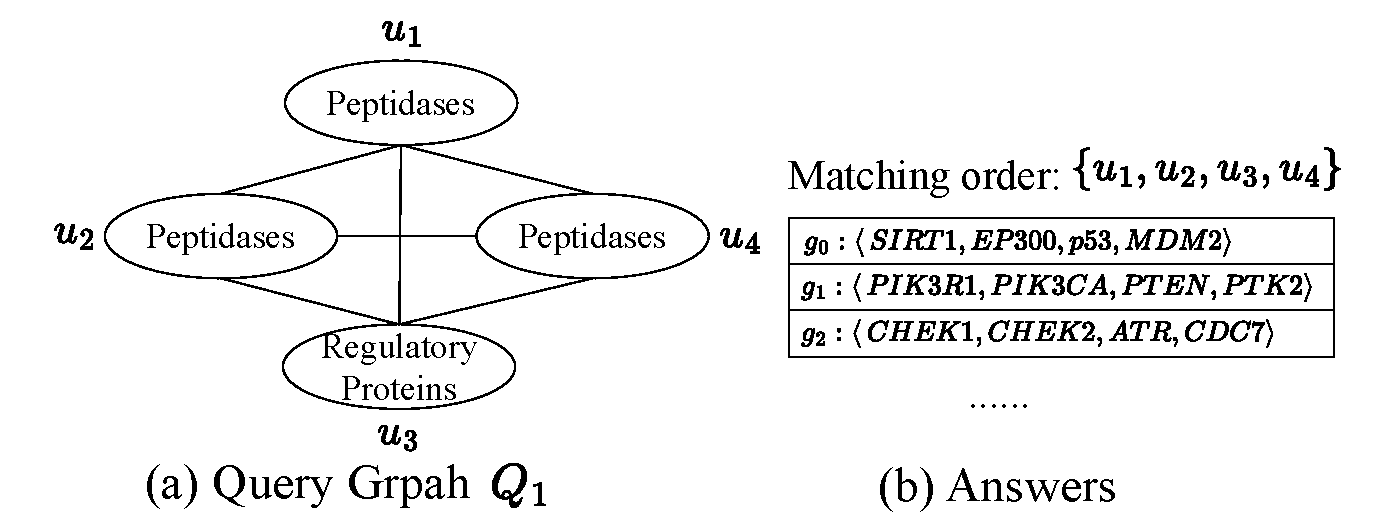
\includegraphics{./exp/newFIg/human_casestudy.pdf}
    }
    \caption{基于蛋白质相互作用网络的案例研究}
    \label{fig:human-caseStudy}
    \end{figure}    
图 \ref{fig:human-caseStudy} 展示了一个查询图 $Q_1$ 及其在蛋白质相互作用网络~\cite{dat-protein} 中的查询结果。
    $Q_1$ 表示由一个调节蛋白和3个肽酶组成的关键结构,边的权重表示相互促进或抑制的程度。
    我们根据边的权重优先排序关系,以识别与相互作用度最高的前 $k$ 个子图。
    在匹配顺序 ${u_1, u_2, u_3, u_4}$ 下,最密集的答案是 $g_0=${$SIRT1$, $EP300$, $p53$, $MDM2$}。
    请注意,$p53$ 是在人类细胞中广泛研究的肿瘤抑制蛋白,而其他三个蛋白激酶表现出强烈的相互作用,并对 $p53$ 产生显著的促进作用,这可能与肿瘤疾病的状态密切相关。
\section{本章小结}
本章详细介绍了我们提出的算法的实验设计与结果分析。
首先介绍了实验环境与配置,包括硬件和软件平台的详细信息、五个真实数据集、查询图的生成方式、以及参与测试的算法。
在实验中,我们通过从数据图中随机抽取子图生成查询图,并对不同查询图大小和不同的$k$值进行了全面测试。
接着,我们对实验结果进行深入分析,通过对比不同算法的时间和空间效率,证明与其他已有的解决方案相比,我们的方案在插入和删除效率上,比其他方案快2-4个数量级,这验证了我们的优化方法在处理大规模数据集时的优势。
同时,我们对比了我们自己提出的四种算法,分别是基线算法、全局MWstar算法、全局与局部MWstar结合的算法以及最终提出的压缩图上的MWstar算法。
实验结果表明,我们的最终算法显著优于基线方法,提升了$1\sim2$个数量级。此外,基于MWstar的全局和局部索引方法也表现出明显的性能优势,尤其是在搜索效率方面,证明了我们算法的有效性和优越性。
最后,我们还给出了CSM-TopK问题在蛋白质相互交互网络上的案例研究,验证了此算法的应用研究价值。
\begin{summary}
	近年来,随着大规模图数据在各个领域的广泛应用,图计算技术逐渐成为研究的热点,尤其是在智能交通、社交网络、金融风控等领域中,如何高效处理图数据和解决实际问题的挑战变得愈发重要。
	子图匹配作为图计算中的关键问题,尤其是在复杂图结构中进行快速的子图匹配计算并获取所有的子图匹配结果,已成为研究的热点。
	由于动态图相比静态图具有更高的应用价值,因此连续子图匹配(CSM)问题更是学术界和工业的关注重点。

	尽管国内外已有多个优秀团队在连续子图匹配问题上进行深入研究,提出了多种优化策略并取得了显著成果,
	但现有的CSM方法普遍忽略了一个重要问题:在大规模数据图下,子图匹配的结果数目庞大,密度优先级机制在筛选有价值的子图匹配结果中起到至关重要的作用。
	此外,尽管已有研究在静态场景下提出了利用密度优先级筛选TopK子图的方法,但由于其索引结构的构建时间和空间复杂度呈指数级增长,离线构建时间长,无法有效应用于CSM问题。
	
	针对以上问题,本文提出了一种新的子图匹配问题——CSM-TopK(密度约束下的TopK连续子图匹配问题),并设计了一种基于密度剪枝的高效算法。本文的研究成果主要集中在以下几个方面:
		
		(1) 本文首先通过形式化定义子图匹配、密度等核心概念,建立CSM-TopK的基础计算框架,首次提出了在子图匹配算法的递归搜索过程中与密度优先级机制相结合的基线方法。提出了基于第$k$个子图匹配结果的密度上限,不再维护第$k$个之外的子图匹配结果。通过引入密度优先级机制,可以筛选出更有价值的匹配结果供数据分析人员进一步分析。

		(2) 为了更高效的解决CSM-TopK问题,本文设计了一种轻量级的星形索引结构。基于该索引结构扩展出两种关键索引——全局MWstar和局部MWstar索引,分别通过维护全局和局部匹配的密度上限,有效减少不满足密度约束的搜索空间,从而优化计算过程。
		首先,全局MWstar索引为子图匹配的递归搜索过程提供了一种粗粒度的密度上限$gBound$,显著减少了无效的搜索空间;其次,局部MWstar索引在全局索引的基础上进一步缩小候选集合,构建了更为紧凑的密度上限$lBound$,可以更早的发现无意义的搜索路径,减少部分子图匹配的递归深度。
		更重要的是,我们构建的全局和局部的星形索引能够保持常数的时间复杂度和线型的空间复杂度,既有效减少了计算时间,也降低了空间消耗,确保了在大规模图数据中的高效性。

		(3) 为了进一步提升算法的效率,本文引入了图压缩技术,通过NLF标签过滤策略构建了规模更小的压缩图,显著降低了计算和存储的负担。
		此外,压缩图在压缩原数据图的大小规模的基础上,继续维护MWstar索引,从而实现了比基线方法更严格的密度上限。该算法在处理动态数据更新时,能够保持较低的时间复杂度和空间复杂度,适应了大规模图数据中的复杂需求。
		
		(4) 本文所提出的算法在五个真实的数据集上进行多组循环测试,验证了所提出的密度剪枝算法的有效性。
		实验结果表明,我们的最终算法——基于压缩图上的MWstar索引剪枝算法,相较于其他已有的解决方案,能够显著提高查询效率,性能提升达到2至4个数量级。
		随着数据集规模的增大,其算法的性能提升更为显著。
		%此外,我们还对比了我们的方案中与其他方案的索引的构建时间以及空间开销,实验证明我们的索引的轻量级。
		此外,我们还对比了本文提出的四种优化算法之间的性能差异,验证了所提索引的轻量级特性。与基线方法相比,图压缩技术和MWstar索引剪枝策略在算法性能上提升了1至2个数量级。
		因此,我们可以得出结论,我们的算法在处理大规模图数据时,能够有效节约计算时间和空间资源。
	
	本文重点研究密度约束下的TopK连续子图匹配问题,旨在图数据中实时高效的查询匹配查询图的前k个密度最大的匹配结果。在研究的过程中,本文考虑到了动态场景下更新的复杂程度,基于动态场景提出了适应于动态场景的索引结构,大大提升了算法的时空效率。
	尽管本文在CSM-TopK问题的研究中取得了初步成果,但仍有许多方面可以进一步优化。未来的研究方向可以从以下几个方面进行扩展:

		(1)子图匹配的多样性研究:
		当前的CSM-TopK算法可能返回彼此之间重叠程度比较高的匹配结果,
		但在实际应用中,如何保证返回结果的多样性,是一个值得进一步研究的方向。
		未来的研究可以引入多样性约束,探索如何在密度约束下返回重叠程度更低的前$k$个匹配结果,以提高算法的实用性,尤其在社交网络分析和推荐系统中,能够更好地满足用户的个性化需求。

		(2)更多约束条件的引入:本文研究的主要集中于子图的密度优先级约束,但在实际应用中,可能还需考虑时间成本、空间成本等其他约束条件。
		未来的研究可以结合用户的个性化需求,将这些约束条件融入密度的计算公式中,通过加权融合不同约束条件的密度公式,从而进一步提升匹配结果的准确性和优化性。

		(3)硬件加速与算法优化:本文提出的优化算法都是基于软件层面的优化,而软件与硬件的协同优化更能够推动技术的进步与发展,因而在未来的研究中可以考虑将算法与现代硬件加速相结合。
		例如,利用图形处理单元(GPU)或现场可编程逻辑门阵列(FPGA)等硬件设备的并行计算能力,将子图匹配的搜索过程并行化处理,从根本上提升计算速度和算法效率。特别是在面对大规模的图数据时,硬件加速能够显著改善处理能力。

		(4)密度上限的进一步优化:在大规模稠密数据图中,一个查询图可能会产生亿万级别的子图匹配结果,如何设计高效的索引结构以得到更严格的密度上限,成为了优化CSM-TopK问题的关键。
		因此,未来研究可以在现有轻量级索引结构的基础上,进一步缩小匹配序列中的候选点的范围,以获得比当前方法更加严格的密度上限,提前剪枝无用扩展过程,减少了递归的深度,从而提高查询效率和可扩展性。

	综上所述,本文提出的CSM-TopK问题及其基于MWstar的密度剪枝算法,在子图匹配中取得了显著进展,尤其在动态大规模图数据处理中展现了较高的效率和可行性。
	尽管目前仍面临一些挑战,未来的研究可以从多样性研究、约束条件引入、硬件加速与算法优化、密度上限优化等多个方向进行深入探索,以促进该算法在实际应用中的广泛落地与发展。
\end{summary}

\bibliography{references}

\appendix
\chapter{读学位期间所发表的学术论文}

\begin{enumerate}[label={[\arabic*]},leftmargin=*,align=left]
    \item \textbf{Chuchu Gao}, Youhuan Li, Zhibang Yang, Xu Zhou. 
    \textsf{CSM-TopK: Continuous Subgraph Matching with TopK Density Constraints}. 
    In \textit{Proceedings of the 40th IEEE International Conference on Data Engineering (ICDE)}, 
    Utrecht, The Netherlands, May 13-16, 2024, pp. 3084-3097. IEEE, 2024. 
    DOI: \href{https://doi.org/10.1109/ICDE60146.2024.00239}{10.1109/ICDE60146.2024.00239}
    
    \item (专利)\textbf{周旭},\textbf{高楚楚},杨志邦,李友焕,杨圣洪,肖国庆,李肯立. 
    \textsf{一种基于动态加权图的Top-k密集子图匹配方法和系统}. 
    国家发明专利,申请号 202311708146.7
\end{enumerate}

\chapter{读学位期间所参加的科研项目}

\begin{enumerate}
    \item 行业知识图谱自动构建与生命周期管理技术,科大讯飞股份有限公司,项目批准号: 2021YFF0901002,研究年限:2021年12月-2024年11月。
\end{enumerate}


\backmatter
\begin{acknowledgements}
	不知不觉中,在湖南大学计算机科学与技术专业攻读硕士的岁月也即将画上句号。回首这三年,我的心态发生了很大的变化。
	研一刚入学时,我的心中充斥着焦虑和后悔。由于研一后互联网的就业步入了寒冬,看着本科人均大厂的同学,我心中有悔。
	同时,面对着未知的研究生生涯,我总是产生一阵又一阵的焦虑情绪,我害怕研究生三年虚度光阴,我害怕浑浑噩噩的度过而一事无成。
	但是,我遇到了很多很美好的人,他们治愈、关怀、鼓励着我;渐渐地,我变得越来越珍惜这段校园时光,三年一晃而过,而现在我的心中只有着感恩和不舍。
	在此,我希望以我最真挚的笔触,向一路给予我帮助的大家表达谢意。

	师者之光。首先,我要重心的感谢我的两位导师周旭老师和李友焕老师。很幸运,我的三年有两位这么优秀的老师共同指导。
	周旭老师给人的感觉就是平易近人、和蔼可亲,不管是学业上还是工作上,都给予着我很大的帮助。
	她教会了我“努力比天赋更加重要”,让我明白了,每日勤勤恳恳的努力,终将会有回报。
	而李友焕老师,则可以说是我科研以及人生道路上的引路人,不仅是教会了我科研的技巧,也教会了我很多为人处事之道。
	从本科毕设开始,李老师就一直亲力亲为,远程和我讨论课题,一谈就是一个小时。硕士期间,从科研选题的确定到具体算法的实现,
	以及论文的撰写,都离不开李老师的悉心指导。从每周多次的学术课题讨论,深夜中发消息解答我的疑问,科研遇到瓶颈时的鼓励以及帮助,
	论文中每句话的逐句斟酌,无不让我感觉科研的严谨和温度。抛开科研,在就业指导方面,李老师也像一束光一样照亮了我前方的迷惘。他会花时间一句句修改我的简历,
	会时常关心我的就业进展,也会关心我的心情和状态。最终,我能拿到不错的工作,这也离不开李老师的一直以来对我的帮助。
	总之,非常感谢两位老师在科研学习、项目实验中的倾囊相授,愿您们学术长青,桃李满天。
	
	同窗之谊。非常感谢一路上陪伴共同学习生活的418和547的小伙伴们,你们的陪伴让我觉得科研枯燥的日子中也有了一些乐趣和珍贵。
	感谢我的好同门们,和你们互相的倾诉、聊天,分享着生活中的趣事,让我觉得研究生的科研之路都不再是孤身奋战,而是互助友爱。
	这三年来,大家每天在实验室一起学习、干饭、爬山、玩桌游、探索了湖大周围好多好吃的小店。
	非常感谢研究生三年有你们陪我一起疯狂,希望现在短暂的离别,只是为了未来我们更好的相聚。
	
	同室之情。非常感谢本科605宿舍的小伙伴们,我们的同宿舍的情谊一直延续至今。感谢你们在我压力大的时候给予我的鼓励,
	在我委屈的时候也一直站在我的角度上安慰我。虽然我们大家因为读研和工作各奔东西,但是大家每天都会在群上分享自己每天琐事,
	就好像回到了宿舍半夜我们仍然叽叽喳喳,熄灯长谈的时候。希望你们未来都能在各自的领域里闪闪发光。
	
	相知相守。在此特别感谢我的男朋友。异地给我们的感情带来的重大的挑战,但是你总是在无数个节假日和周末义无反顾的奔向我。
	每当我遇到心情不好的时候,总是把自己的坏情绪第一时间的反馈给你。无数的日夜,你总是不厌其烦的听我诉说着生活中的喜怒哀乐。
	祝愿你在未来的日子里学术坦途,而我们继续相伴前行。

	父母之恩。在此要感谢我的家人们,他们成为了我坚强的后盾,让我能心无旁骛的做我想做的事情。虽然他们不懂我的研究生要做什么,
	但是也总是会默默倾听我的牢骚,偷偷了解我的研究方向,特别是我的弟弟妹妹,在我心情不好的时候,总是第一时间“使相”,用力搞笑逗我开心。
	希望你们都能平安健安,希望以后的我能成为你们的后盾。

	不负韶华。最后,我要感谢一直没有放弃的自己。感谢自己的三年没有虚度光阴,感谢无数个挑灯夜战的日子,感谢无数次想要放弃却又继续坚持的时刻。
	“宝剑锋从磨砺出,梅花香自苦寒”,愿自己能成为那一把宝剑,那一缕寒梅,不惧磨砺,不畏严寒。

	麓山巍巍,湘水汤汤。行文最后,谨谢母校湖南大学,我将时刻谨记“实事求是,敢为人先”的校训,
	未来我将以务实创新的态度投身技术领域,不负湖大所育。

\end{acknowledgements}


\end{document}
